\documentclass[11pt,a4paper,oneside,extrafontsizes]{memoir}

\renewcommand*{\baselinestretch}{1.04}
\isopage
\setlrmargins{*}{*}{1}
\checkandfixthelayout
%\documentclass[11pt,a4paper,twoside,openright,extrafontsizes]{memoir}

\renewcommand*{\baselinestretch}{1.04}
\isopage
\checkandfixthelayout
\usepackage{include/thesis}

\newcommand*{\bme}{Budapest University of Technology and Economics}
\newcommand*{\vik}{Faculty of Electrical Engineering and Informatics}

\newcommand*{\bmemit}{Department of Measurement and Information Systems}

\newcommand*{\vikdoctype}{Master's Thesis}
\newcommand*{\viktdkyear}{2016}

\newcommand*{\authors}{Author}
\newcommand*{\advisors}{Supervisors}

\newcommand*{\authori}{Dániel Stein}

\newcommand*{\advisori}{Gábor Szárnyas}
\newcommand*{\advisorii}{Ádám Lippai}
\newcommand*{\advisoriii}{Dávid Honfi}

\title{Graph-Based Source Code Analysis of JavaScript Repositories}
%\newcommand*{\titlepagetitle}{Graph-Based\\Source Code Analysis\\of JavaScript Repositories}
\newcommand*{\titlepagetitle}{Graph-Based\\Source Code Analysis\\of Dynamically Typed Languages}
\author{\authori}

\hypersetup{
  pdftitle={\thetitle},
  pdfauthor={\theauthor, \advisors: \advisori, \advisorii, \advisoriii}
  bookmarks=true,            % show bookmarks bar?
  unicode=true,              % non-Latin characters in Acrobat's bookmarks
  pdfnewwindow=true,         % links in new window
  colorlinks=true,           % false: boxed links; true: colored links
  linkcolor=black,           % color of internal links
  citecolor=black,           % color of links to bibliography
  filecolor=black,           % color of file links
  urlcolor=black             % color of external links
}


%\usepackage{marginnote}
%\usepackage{epigraph}
\usepackage[shortlabels]{enumitem}
\usepackage{placeins}
\usepackage{adjustbox}
\usepackage{booktabs}
\newcommand{\code}[1]{{\upshape\ttfamily\small\indent #1}}

\graphicspath{ {./include/figures/}, {./include/sources/} }

\usetikzlibrary{automata,arrows,positioning,trees,shapes.geometric}
\tikzset{
	>=stealth',
	stdstage/.style={
		rectangle,
		rounded corners,
		draw=black,
		minimum height=2.5em,
		text centered},
	processor/.style={
		diamond,
		minimum width=2em,
		minimum height=2em,
		aspect = 1,
		draw = black
		},
	flowedge/.style = {
		->,
		>=stealth',
		shorten >=1pt
	},
	textedge/.style={
		draw=none,
		text width = 7.5cm,
    inner sep = 1cm,
		align = left
	}
}


\usepackage{listings}
\lstset{
	basicstyle=\scriptsize\ttfamily, % print whole listing small
	keywordstyle=\color{black}\bfseries, % bold black keywords
	identifierstyle=, 					% nothing happens
	commentstyle=\color{gray},
	stringstyle=\scriptsize,
	showstringspaces=false,     % no special string spaces
	aboveskip=1em,
	belowskip=3pt,
	columns=flexible,
	backgroundcolor=\color{white},
    extendedchars=false,
    inputencoding=utf8
}
\lstset{xleftmargin=1em,
        framexleftmargin=1em,
        framextopmargin=1em,
        framexbottommargin=1em,
        frame=tb, framerule=0pt}
\lstset{escapeinside={(*@}{@*)}}
\def\lstlistingname{Source}

% source: http://tex.stackexchange.com/questions/83085/how-to-improve-listings-display-of-json-files
\usepackage{xcolor}

\colorlet{punct}{red!60!black}
\definecolor{delim}{RGB}{20,105,176}
\colorlet{numb}{magenta!60!black}

\lstdefinelanguage{json}{
    basicstyle=\normalfont\ttfamily,
    showstringspaces=false,
    breaklines=true,
    frame=lines,
    literate=
     *{0}{{{\color{numb}0}}}{1}
      {1}{{{\color{numb}1}}}{1}
      {2}{{{\color{numb}2}}}{1}
      {3}{{{\color{numb}3}}}{1}
      {4}{{{\color{numb}4}}}{1}
      {5}{{{\color{numb}5}}}{1}
      {6}{{{\color{numb}6}}}{1}
      {7}{{{\color{numb}7}}}{1}
      {8}{{{\color{numb}8}}}{1}
      {9}{{{\color{numb}9}}}{1}
      {:}{{{\color{punct}{:}}}}{1}
      {,}{{{\color{punct}{,}}}}{1}
      {\{}{{{\color{delim}{\{}}}}{1}
      {\}}{{{\color{delim}{\}}}}}{1}
      {[}{{{\color{delim}{[}}}}{1}
      {]}{{{\color{delim}{]}}}}{1},
}

% source: http://tex.stackexchange.com/questions/89574/language-option-supported-in-listings
\lstdefinelanguage{JavaScript}{
  basicstyle=\normalfont\ttfamily,
  keywords={break, case, catch, continue, debugger, default, delete, do, else, finally, for, function, if, in, instanceof, new, return, switch, this, throw, try, typeof, var, void, while, with},
  morecomment=[l]{//},
  morecomment=[s]{/*}{*/},
  morestring=[b]',
  morestring=[b]",
  sensitive=true
}

\lstdefinelanguage{Cypher}{
  morekeywords=[1]{BY, CREATE, DELETE, FOREACH, LIMIT, MATCH, MERGE, OPTIONAL, ORDER, REMOVE, RETURN, SET, SKIP, UNIQUE, WHERE, WITH, AND, OR},
	morekeywords=[2]{(, ), [, ], -(, )-, -[, ]-, --, ->, <-, -->, <--, )-->, )<--, -->(, <--(},
	keywordstyle={[2]\color{delim}},
  morecomment=[l]{//},
  morecomment=[s]{/*}{*/},
  morestring=[b]',
  morestring=[b]",
  sensitive=true,
	literate=
	 *{0}{{{\color{numb}0}}}{1}
		{1}{{{\color{numb}1}}}{1}
		{2}{{{\color{numb}2}}}{1}
		{3}{{{\color{numb}3}}}{1}
		{4}{{{\color{numb}4}}}{1}
		{5}{{{\color{numb}5}}}{1}
		{6}{{{\color{numb}6}}}{1}
		{7}{{{\color{numb}7}}}{1}
		{8}{{{\color{numb}8}}}{1}
		{9}{{{\color{numb}9}}}{1}
}

\bibliography{bibliography}

\begin{document}

\frontmatter{}

\thispagestyle{empty}

\begin{tikzpicture}[overlay,remember picture]
  \node at (current page.center) [yshift=1cm] {%
    \begin{minipage}{\textwidth}

      \centering

      
\includegraphics[width=7cm]{include/figures/bme_logo}
      \vspace{0.3cm}

      \bme \\
      \vik \\
      \bmemit \\
      \vspace{3.5cm}

      {\Huge\sffamily\bfseries \titlepagetitle \par}
      \vspace{1cm}

      {\large \vikdoctype \par}
      \vspace{2cm}

      {\Large
        \authors: \\ \vspace{0.3cm}
        \authori

        \vspace{1cm}
        \advisors: \\ \vspace{0.3cm}
        \advisori \\
        \advisorii\par}

      \vspace{1.5cm}
      {\large \viktdkyear.\par}

    \end{minipage}};
\end{tikzpicture}

\cleardoublepage

\tableofcontents

\selectenglish{}
{
\selecthungarian{}
\begin{center}
\large
\textbf{HALLGATÓI NYILATKOZAT}\\
\end{center}

Alulírott \emph{Stein Dániel}, szigorló hallgató kijelentem, hogy ezt a diplomatervet meg nem engedett segítség nélkül, saját magam készítettem, csak a megadott forrásokat (szakirodalom, eszközök stb.) használtam fel. Minden olyan részt, melyet szó szerint, vagy azonos értelemben, de átfogalmazva más forrásból átvettem, egyértelműen, a forrás megadásával megjelöltem.

Hozzájárulok, hogy a jelen munkám alapadatait (szerző(k), cím, angol és magyar nyelvű tartalmi kivonat, készítés éve, konzulens(ek) neve) a BME VIK nyilvánosan hozzáférhető elektronikus formában, a munka teljes szövegét pedig az egyetem belső hálózatán keresztül (vagy autentikált felhasználók számára) közzétegye. Kijelentem, hogy a benyújtott munka és annak elektronikus verziója megegyezik. Dékáni engedéllyel titkosított diplomatervek esetén a dolgozat szövege csak 3 év eltelte után válik hozzáférhetővé.

\begin{flushleft}
\vspace*{1cm}
Budapest, \today
\end{flushleft}

\begin{flushright}
 \vspace*{1cm}
 \makebox[7cm]{\rule{6cm}{.4pt}}\\
 \makebox[7cm]{\emph{Stein Dániel}}\\
 \makebox[7cm]{hallgató}
\end{flushright}
\thispagestyle{empty}

\vfill
\clearpage
\thispagestyle{empty} % an empty page

}

\begin{otherlanguage}{magyar}

  \paragraph*{Kivonat}
  \phantomsection
  \addcontentsline{toc}{chapter}{Kivonat}
  \thispagestyle{plain}
  {
  \selecthungarian

  Egyre több, egyre inkább komplex szoftver vesz körül minket, sok esetben ezek akár részét képezhetik kritikus rendszereknek is. Az ilyen rendszerek fő jellemzője, hogy a legapróbb hibáik is komoly következményekkel járhatnak. A forráskód statikus analízise egy, a kritikus szoftverrendszereknél általánosan elfogadott megközelítés, amely a hibák mihamarabbi megtalálását célozza meg.  A statikus analízis már a fejlesztési folyamat korai szakaszaiban is alkalmazható, mivel nincs szükség a kód fordítására és futtatására az ellenőrzés véghezviteléhez. A megközelítést számos eszköz megvalósítja, amelyek képesek visszajelzést adni a potenciális hibahelyeken túl arról is, hogy a forráskód megfelel-e a kódolási szabályoknak és követelményeknek.

  Habár több statikus analízis eszköz is elérhető generikus nyelvek elemzéséhez, és ezek többsége beépíthető a folytonos integráció folyamatába is, JavaScript esetén ez nem mondható el annak dinamikus volta végett. A dinamikus nyelvek sajátosságai miatt csak pár eszköz érhető el JavaScript forráskódok kódtárszintű statikus analíziséhez, illetve az eddig ismert ilyen eszközök nem nyújtanak egyszerre megoldást alaki ellenőrzésre, futási utak meghatározására és folytonos integrációba történő integrációra.
  
  Jelen dolgozatomban egy olyan, a folytonos integráció kiegészítésére képes keretrendszert tervezek, valósítok meg és értékelek, amely képes nagyméretű és gyakran változó JavaScript forráskódtárak konfigurálható statikus analízisére. A keretrendszer alapjául szolgáló újszerű megközelítésnek köszönhetően az eddig megszokott megoldások helyett a felhasználók egyszerűbb módon fejezhetik ki az ellenőrzésre szánt követelményeket és képesek a több forráskódon átívelő követelményeket hatékonyabban elemezni.

  }

\end{otherlanguage}

\cleardoublepage

\paragraph*{Abstract}
\phantomsection
\addcontentsline{toc}{chapter}{Abstract}
\thispagestyle{plain}

We are surrounded by more and more complex software that operate in mission-critical systems. Even small errors in these software can lead to consequences ranging from unpleasant to expensive. A proven approach for detecting mistakes early in the development cycle is static analysis of the source code. Static analysis tools report whether the software conforms to the coding rules and requirements without executing the code itself.

While multiple static analysis tools exist for general purpose programming languages and these are generally part of the continuous integration systems, this is not the case with JavaScript. Because of the untyped nature of this dynamic language there are only a few tools that perform static analysis on JavaScript code repositories on a global level.

In this report I design, implement and evaluate a framework aiming to extend the continuous integration workflow of large JavaScript repositories with various static analysis tools and techniques.

\clearpage

\newcounter{savepage}
\setcounter{savepage}{\arabic{page}}

\mainmatter{}

\chapter{Introduction}
\label{chap:introduction}

\section{Context}

Quality control plays an important role in large-scale software development. The number of coding errors are noticeably increasing with the number of contributors. The more developers work together on developing a software, the more versatile their coding styles and conventions are.

To ensure the quality of the source code, thus the software itself, and at the same time help developers with their tasks, the need arises for a solution continuously reviewing the code, searching for mistakes, and enforcing conventions.

\begin{figure}[!ht]
	\centering
	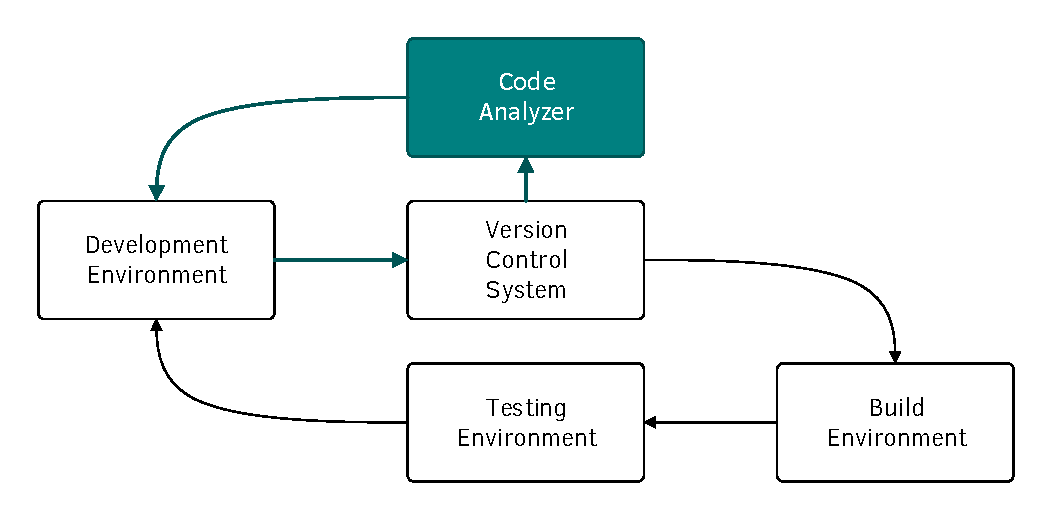
\includegraphics[height=6cm]{CI-workflow}
	\caption{Continuous Integration workflow extended with Static Analysis.}
	\label{fig:CI-workflow}
\end{figure}

Version control systems (VCS) and continuous integration (CI)~\cite{CI} are widely used tools of the modern software developers. \Cref{fig:CI-workflow} shows an extended version of the generally used continuous integration workflow.
The basic workflow consists of the following steps. The developer makes modifications to the codebase using their \textit{Development Environment}. The modifications are committed into a \textit{Version Control System}, and this commit triggers the \textit{Build Environment} to build the project. The \textit{Testing Environment} can then perform runtime tests on latest build of the project. After this process, the results --- build and test logs --- are presented to the developer.

These logs help the developers discover bugs and failures before the software is released for manual testing or production purposes. Producing this information and making sure the software is working as intended often and early in the development workflow is vital for agile development.

A proven method of enhancing software quality is utilizing static program analysis techniques supplementing the basic CI workflow. During this method, the code is analyzed without executing the application. In practice, this method is able to reveal problems that are undetectable with testing and thus is able to aid the developer in creating higher quality software.


\section{Problem Statement}

Static analysis methods verifying that the code is compliant with coding conventions are often time consuming and resource intensive in practice. The size of the codebase may require a scalable solution, especially for continuous integration purposes, since the entire verification process needs to be carried out on the whole codebase once it is (partially) modified.

A temporary solution to tackle this problem is to process the changes in batches. To save resources, static analysis runs are carried out for a joined group of changes, rather than for every individual commit.

In an ideal situation, even before committing the changes, the developers receive feedback about the problems their modifications would imply.


\section{Objectives and Contributions}

My main objective is to provide a solution for reducing the time required for global, codebase-level reevaluation of static analysis after a change occurs.

I aim to create a framework that transforms the whole source code repository into a graph representation and maintains it subsequently. It should perform code convention compliance checks, execute built-in static analysis tests and be extended with arbitrary tests by the user.

Incremental processing is one of the possible solutions for speeding up static analysis. Thus it should be able to process a subset of the repository, e.g. only the modifications introduced by the latest commit, then integrate the changes into the maintained representation. This way the system can process the modifications in a commit incrementally. After the initial query evaluation and report generation, consecutive runs can be executed significantly more efficiently.

The framework relies on two substantial technologies --- a source code parser and an adequate database solution --- and provides interfaces making integration possible with external tools, such as version control systems and integrated developer environments.


\section{Structure of the Thesis}

This thesis is structured as follows.
\Cref{chap:preliminaries} introduces the previously mentioned background technologies required and selected to build an incremental static analyzer.
\Cref{chap:background-and-related-work} details the various approaches and related researches.
\Cref{chap:overview-of-the-approach} shows the overview of my approach and gives detailed view of the main components of its architecture.
\Cref{chap:elaboration-of-the-workflow} presents the implementation of the framework, and discusses the steps of the analysis.
\Cref{chap:evaluation-of-the-prototype} demonstrates and evaluates the performance of the framework.
\Cref{chap:future-vision} reveals future vision ideas and possibilities.
\Cref{chap:conclusions} concludes the thesis.

% !TEX root = ../main.tex
\chapter{Preliminaries}
\label{chap:preliminaries}

In this chapter I present the conceptual foundations and related technologies of my work. Also, I discuss the building blocks required to design a static analyzer framework for JavaScript.

\section{JavaScript}
Ohe most used dynamic languages in the world is JavaScript. According to~\cite{js-usage}, JavaScript is the most utilized client-side programming language for web applications, with over 94\% estimated usage. In this section I briefly summarize the history of JavaScript, present recent advancements and discuss why it is timely to utilize static analysis techniques for the language.

\subsection{From Glue Language to a Full-Fledged Language}
This section follows~\cite{10.1109/MC.2012.57}. The language written in 10 days by Brendan Eich in April 1995 --- originally called LiveScript --- was one of the first attempts at bringing dynamic behavior to the web. It was supposed to look like Java, leaving its complexity behind and appealing for developers looking for easy scripting solutions on the web.

The initial goal --- to create a language for portable applications --- has been seemingly achieved by the time of writing this report. While it has been gaining popularity due to its simpler syntax, the language, its tooling, and its community had time to evolve, making it the most used web programming language. JavaScript has shifted from simpler scripts to complex systems on the web, desktops, and servers.

\subsection{ECMAScript}
\label{sect:ecmascript}
After its release, JavaScript was submitted to and standardized by the Ecma International industry association, resulting in the first release of the ECMAScript language specification (of the ECMA-262 standard~\cite{ecma-262}) in June 1997. Apart from JavaScript, there are several implementations, e.g., \emph{Chakra}\footnote{\small\url{https://github.com/Microsoft/ChakraCore}}, \emph{JScript}\footnote{\small\url{https://msdn.microsoft.com/library/hbxc2t98.aspx}}, and \emph{V8}\footnote{\small\url{https://github.com/v8/v8}}.

There are several reasons why the standard and the usage of ECMAScript is getting more and more popular. Besides the improvement of the developer tools, developer community, and being already popular, conscious and regular development of the language also makes the language more appealing. At the time of writing this report there are 8 editions of the standard, 6 of them published. The last published edition, ES7 was published in June 2016, one year after the previous edition, ES6.

The initial language specifications were indulgent, and only best practices were guiding the developers. The challenges of analyzing such dynamic, untyped language --- able to express one thing in several different ways --- may be one of the reasons why there are only a few tools present even today implementing static analysis for ECMAScript.

The syntactic sugars added to the language across the editions of ECMAScript made it possible to express the most used code parts in an easier manner, while being more concise. Encouraging the developers to use these constructs makes it easier to interpret the source code --- both manually and with source code analysis.

% \subsection{Emerging Languages Translating to JavaScript}
% \subsubsection{WebAssembly}


\section{Static Analysis}
The idea of static analysis is almost half a century old. A paper from 1995 states that \textquote[\cite{wichmann_industrial_1995}]{The idea  that computer software should be used to analyze source programs rather than compile them, has a history of at least 25 years.}

Source code analysis can be used to discover facts about a particular program. Two basic automated analysis methods exist for this purpose:
\begin{itemize}[topsep=0pt]
  \item \emph{Static analysis} is performed by parsing the source code and analyzing it without evaluating the statements or executing the program.
  \item \emph{Dynamic analysis} is performed by executing the program and evaluating its output for given input sequences.
\end{itemize}

% > The term is usually applied to the analysis performed by an automated tool, with human analysis being called program understanding, program comprehension, or code review. Software inspections and Software walkthroughs are also used in the latter case.
% https://en.wikipedia.org/wiki/Static_program_analysis

While high-level language (e.g., C$++$, Java) source codes are checked at least by the compiler, JavaScript is usually not compiled before it is published. Thus a specific static analysis tool for JavaScript should aim to discover unwanted traits of the source in ways a generic compiler would not be able to, resulting in better code quality. These traits, \emph{code smells} are usually perceptible while running the code. Another way to locate these bugs is to write and run tests, dynamically testing the program.~\cite{wichmann_industrial_1995}

The two analysis methods are complementing each other. They discover different subsets of problematic constructions. While static analysis can discover syntactical problems (like the lack of the default case in a switch), dynamic analysis may catch behavioral problems (such as error handling and timing errors). Information discovered using static analysis may be used later in dynamic testing, resulting in a hybrid technique.

% > Static analysis bug-finding tools have evolved over the last several decades from basic syntactic checkers to those that find deep bugs by reasoning about the semantics of code. The goal of the Clang Static Analyzer is to provide a industrial-quality static analysis framework for analyzing C, C++, and Objective-C programs that is freely available, extensible, and has a high quality of implementation.
% http://clang-analyzer.llvm.org/


\subsection{Use Cases}
Static analysis tools employ diverse levels of abstraction. \emph{Formatters} are able to ensure that the source code complies with a predefined style guide. \emph{Linters} check for stylistic and programming errors, thus indicating suspicious programming constructs. \emph{Formal verification}, on the other hand, utilizes formal mathematical methods to prove statements about a piece of source code and its behavior.

For dynamic languages static analysis has even more use cases. For example, it allows finding previously undefined property reads, catching invocation of non-functional variables~\cite{jensen_type_2009}, detecting dead code.

\subsection{Advantages and Disadvantages}
Since static analysis tools deliberately do not evaluate the source code, there are fundamental limitations to what problems they can discover. In the context of my work, static analysis has the following trade-offs.

\subsubsection{Advantages}
\paragraph{No Need for Execution}
Since there is no need for execution, the hardware and software requirements of the analysis software do not need to match the requirements of the application. There is also no need to emulate or mock its dependencies, making the analysis more portable and cost efficient.

\paragraph{Early Detection of Possible Errors}
Static analysis may catch problems even before the whole software is complete or even runnable, potentially allowing the developers to fix the problems earlier in the development process.~\cite{xie}

\paragraph{Thorough}
While dynamic testing executes the manually written or automatically generated test cases covering a portion of the source code, static analysis systematically explores every possible execution scenarios. Thus it may achieve higher coverage and detect more problems in the code.~\cite{xie}

\subsubsection{Disadvantages}
\paragraph{Speed} Static analysis trades CPU time and memory for better code quality. By design it may be multiple orders of magnitude slower than compilation. Its speed depends not only on the underlying data structure and algorithms, but also the level of analysis.~\cite{clang}
% TODO extend

However, with a given limitation of granularity (e.g., considering a single file as the unit of processing), in case of a source code modification, previous results can be reused. There is a possibility that only the modified --- and other affected --- parts need to be processed again. The incremental approach of static analysis may speed up the process by orders of magnitude~\cite{stein-daniel-bsc}.
% TODO clarify

\paragraph{False Positives} Static analysis can not prove the correctness of a source code. It rather warns in case there is a possibility of a problem. Thus static analysis tools can introduce false positive warnings and flag code parts as problematic even if they behave correctly. To reduce the number of false positive warnings, one usually introduces more precise, specified rules and more thorough analysis.~\cite{clang}

\subsection{Source Code Processing and Analysis}
\label{sect:source-code-processing}
The source code of a program is a sequence of instructions formulated in a programming language as a text. Grammars of formal languages are a set of rules describing what the compiler considers a valid input---how to create valid instructions or a set of instructions from the alphabet of the language \emph{(syntax)}. A source code processing entity (transformer, or hereafter \emph{compiler}) assigns a meaning \emph{(semantics)} and transforms the instruction to another language (generally an intermediate language or bytecode).~\cite{Aho:1986:CPT:6448}

What input data the compiler considers useful information depends on the semantics of the language the compiler is built for. Source codes contain a much wider variety of data than a compiler requires for transforming, analyzing the application: comments, function declaration order, indentation, line breaks all help the reader (and writer) of the code, but carry no additional information.

\Cref{fig:processing-the-source-code} shows the general process for processing source code and transforming a stream of characters into a data structure with \emph{meaning} (semantic information).

\begin{figure}[!ht]
	\centering
	\adjustbox{max width=\textwidth} {
		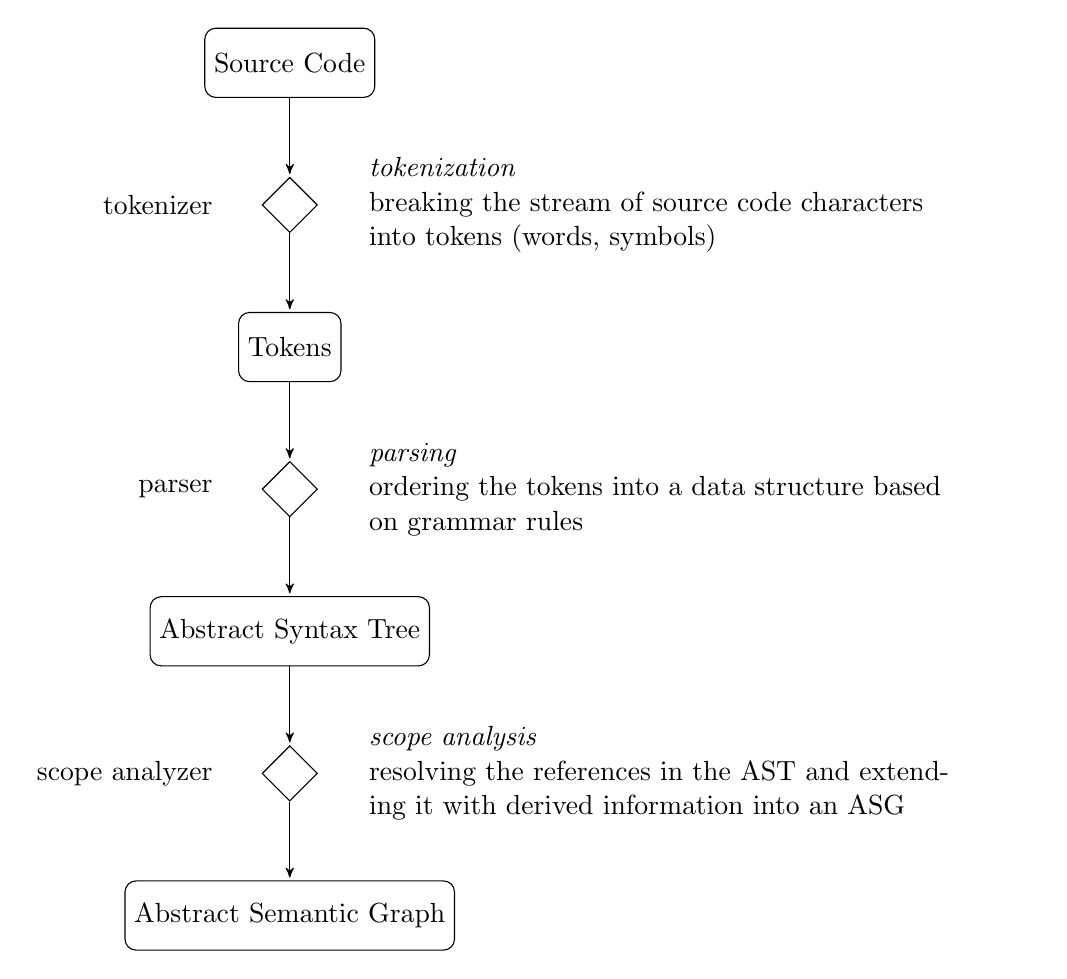
\begin{tikzpicture}[
			node distance = 1cm,
      label distance = 0.5cm,
			auto,
			]

    \node[stdstage] (SC) {Source Code};
    \node[processor,
          below=of SC,
          label={left:tokenizer}
          ] (TOK) {};
    \node[stdstage, below=of TOK] (TO) {Tokens};
    \node[processor,
          below=of TO,
          label={left:parser}
          ] (PAR) {};
    \node[stdstage, below=of PAR] (AST) {Abstract Syntax Tree};
    \node[processor,
          below=of AST,
          label={left:scope analyzer}
          ] (SA) {};
    \node[stdstage, below=of SA] (ASG) {Abstract Semantic Graph};


    \path (SC) edge[flowedge]  (TOK);
    \path (TOK) edge[flowedge] (TO);
    \path (SC) edge[textedge] node {\emph{tokenization}\\ breaking the stream of source code characters into tokens (words, symbols)} (TO);

    \path (TO) edge[flowedge]  (PAR);
    \path (PAR) edge[flowedge] (AST);
    \path (TO) edge[textedge] node {\emph{parsing}\\ ordering the tokens into a data structure based on grammar rules} (AST);

    \path (AST) edge[flowedge]  (SA);
    \path (SA) edge[flowedge] (ASG);
    \path (AST) edge[textedge] node {\emph{scope analysis}\\ resolving the references in the AST and extending it with derived information into an ASG} (ASG);
		\end{tikzpicture}
	}
	\caption{Processing the source code.}
	\label{fig:processing-the-source-code}
\end{figure}

\subsubsection{Lexical Analysis}
A \emph{lexer}, \emph{tokenizer}, or \emph{scanner} forms the first phase of a parsing process. It scans the input character stream and segments them into sequence of groups, tokens, \emph{strings with a ``meaning''}. It also categorizes these groups into various token classes, token types. Processing the raw input into a value (converting the string \code{"2"} into the number $2$) can also happen in this phase. \Cref{fig:tokenization} shows how an expression string can be tokenized.

\begin{figure}[!htb]
  \centering
  \code{foo = 1 / 0}\\[1em]

  \begin{tabular}{c|l}
    Token & Token type\\
    \hline
    \code{foo} & \code{IDENTIFIER (Ident)}\\
    \code{=} & \code{ASSIGN (Punctuator)}\\
    \code{1} & \code{NUMBER (NumericLiteral)}\\
    \code{/} & \code{DIV (Punctuator)}\\
    \code{0} & \code{NUMBER (NumericLiteral)}\\
    \hline
  \end{tabular}

  \caption{Character stream and tokenization result with token type information.}
  \label{fig:tokenization}
\end{figure}


\subsubsection{Parser}
A \emph{parser} forms the second phase of a parsing process, using the output token stream of the \emph{lexer}. It takes the input data and builds a hierarchical data structure (a \emph{parse tree} or an \emph{abstract syntax tree}) representing the input. If the input does not comply with the syntax rules, and a tree can not be built, the source code is syntactically incorrect.

\Cref{fig:sentence-s-expression} shows a sentence and its s-expression representation. S-expressions (for ``symbolic expression'') are a notation for tree-structured nested list, mainly used in Lisp.

\begin{figure}[!htb]
\centering
\code{The quick brown fox jumps over the lazy dog}\\[1em]

\begin{minipage}{3cm}
\begin{verbatim}
(Sentence
  (Word The)
  (Word quick)
  (Word fox)
  (Word jumps)
  (Word over)
  (Word the)
  (Word lazy)
  (Word dog)
)
\end{verbatim}
\end{minipage}
  \caption{A sentence and its s-expression representation.}
  \label{fig:sentence-s-expression}
\end{figure}

\paragraph{Abstract Syntax Tree}
An \emph{Abstract Syntax Tree} (AST) is a tree representation of the syntactic structure of the result of a parsing along a grammar. The nodes of the tree denote a construct occurring in the input, while the edges represent the connection between these nodes based on the grammar rules.

As mentioned in~\cref{sect:source-code-processing}, source code contains much more detail (e.g., indentation, whitespace, comments) than is required and restrained during the parsing process. Thus this representation is a more compact, \emph{abstract} syntax tree. It may be transformed based on transformation rules and source code can be generated from ASTs. Without restraining the layout information and reusing it during the code generation, the resulting text can show differences in indents, whitespaces and expression formulation compared to the initial source code.

\Cref{fig:ast-asg-example} shows an example AST (in black), where a one-statement JavaScript file is parsed. The content of the file was only the following line:

\lstinputlisting[
  language=JavaScript
]{include/sources/oneliner.js}

\subsubsection{Scope Analyzer}
A \emph{scope analyzer} or \emph{context analyzer} produces a data structure that represents the scoping information of a program, extending the information available from an AST or an ASG. An element representing a scope in this data structure may contain, inter alia, metadata about the scope itself, the AST node related to the scope, available assets (variables, functions, etc.) in that scope.~\cite{shift-scope}

\paragraph{Abstract Semantic Graph}
An \emph{Abstract Semantic Graph} (ASG) differs from an Abstract Syntax Tree in two essential concepts: ASGs 1)~are not necessarily trees, and 2)~express more than the syntactic information; ASGs carry semantic information expressed with additional edges. An example of this type of edge connects variable references to their declarations.~\cite{raghavan_dex:_2004}

An ASG is a graph representation of a parse result; the nodes represent subterms of an expression. Shared subterms can occur, having more than one node linked to the same, common subterm. Compilers generally work on ASGs internally, since not only the syntactical, but the behavioral information is also represented in them.

% An abstract semantic graph is typically constructed from an abstract syntax tree by a process of enrichment and abstraction. The enrichment can for example be the addition of back-pointers, edges from an identifier node (where a variable is being used) to a node representing the declaration of that variable. The abstraction can entail the removal of details which are relevant only in parsing, not for semantics.
% https://en.wikipedia.org/wiki/Abstract_semantic_graph

\Cref{fig:ast-asg-example} shows the difference between an AST and an ASG (in turquoise).

\begin{figure}[!htb]
	\centering
	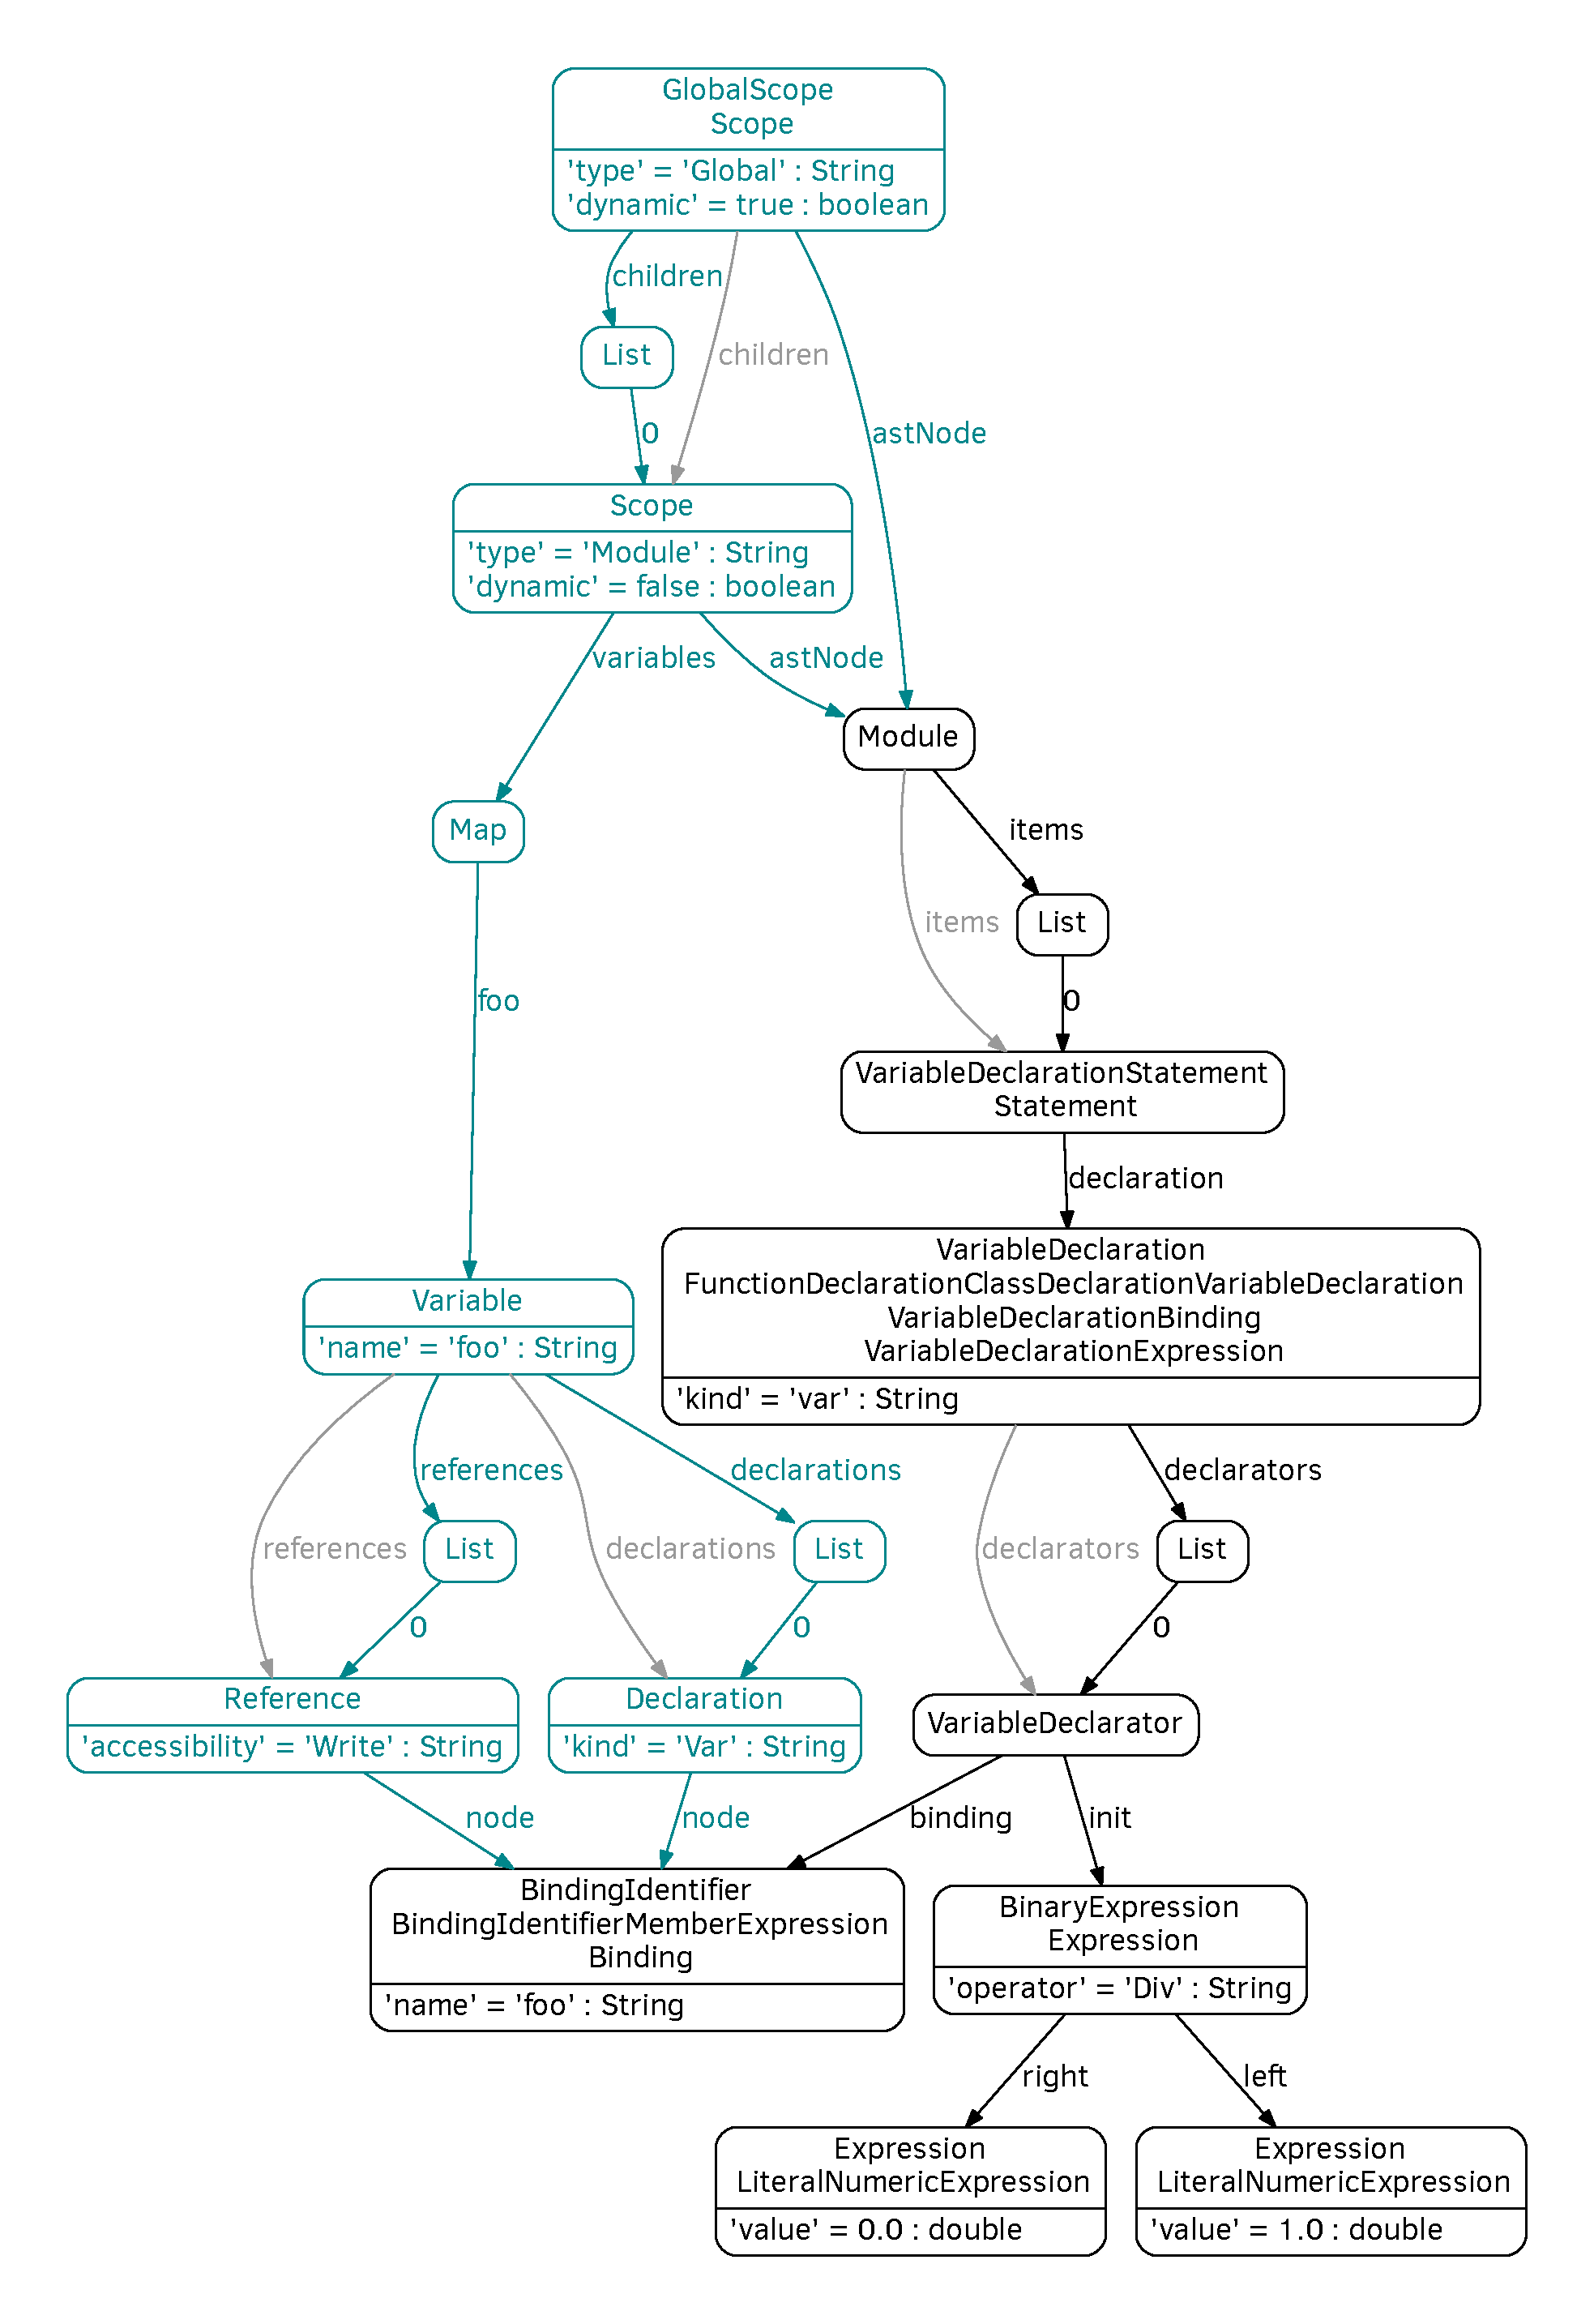
\includegraphics[height=\textheight, trim=1cm 1cm 1cm 1cm,clip]{include/figures/AST-ASG}
	\caption{AST (in black) with additional edges (ASG, in turquoise) and derived helper edges (in gray).}
	\label{fig:ast-asg-example}
\end{figure}

\subsubsection{Type Inference}
\label{sect:introducing-type-inference}
In order to make sure that a system behaves correctly according to the specification, a broad range of \emph{formal methods} can be used. Besides \emph{model checkers}, \emph{run-time monitoring}, the most popular formal methods are \emph{type systems}.~\cite{pierce2002types} \textquote[\cite{pierce2002types}]{A type system is a syntactic method for automatically checking the absence of certain erroneous behaviors by classifying program phrases according to the kinds of values they compute.}

Type inference refers to the deduction of the data types of expressions, statements in the source code, usually executed during compilation and static analysis. By utilizing type inference, deducing types as \emph{interfaces}, and checking contracts --- e.g., preconditions for the types of arguments, postconditions for the types of return values --- between various parts of the software can yield a more consistent and bug-free code.

Type systems also help developers write the source code with context-aware assistance. With implicitly typed languages the ability to infer data types can make prototyping and developing programs occur in a more agile fashion, compared to explicitly typed languages. Omitting the type annotations eliminates the need to propagate changes in the source code in case of a refactor, while still executing interface checks prevent type errors at runtime.

\paragraph{Typed JavaScript Derivations} There are several languages with type systems that compile to JavaScript, such as TypeScript\footnote{\small\url{https://www.typescriptlang.org/}}, Dart\footnote{\small\url{https://www.dartlang.org/}}, Elm\footnote{\small\url{http://elm-lang.org/}}, and Flow.
% TODO ref Flow

%\subsubsection{Tooling}
%There are several static analysis frameworks and solutions available for JavaScript. I introduce and compare them in detail in \cref{sect:javascript-parsers} (JavaScript parsers) and \cref{sect:javascript-type-inferencers} (JavaScript type inferencing solutions).

\FloatBarrier

\section{Handling Large Interconnected Data}
In numerous use cases, interconnected data sets can be represented and processed as a graph. \emph{Graph databases} provide a way to efficiently store graphs and evaluate graph queries. In this section I introduce the concept of graph databases, and graph pattern matching. I also present different types of graph database implementations from which I selected the most appropriate technology for the approach.

The advancements in hardware components -- the ever increasing amount of processing power, and memory and storage speed and sizes -- and the analogous growth of data to be stored and processed during the last more than fifty years yielded various solutions.

Based on historic evolution, these solutions can be categorized in three main categories:
\begin{itemize}[topsep=0pt]
  \item \emph{Navigational} database management systems (DBMS) were mainly used in the era of magnetic tape based storages, in which the \emph{records} contained references to other records allowing the system to fast-forward, \emph{navigate} there and load additional data.

  \item \emph{Relational} DBMSs organizes data in a \emph{relational model}~\cite{codd}, where one or more \emph{relations} contain unique entries (\emph{records} or \emph{tuples}).

  Relational databases leverage precise mathematical background (see \emph{relational algebra} and \emph{relational calculus}), have diverse implementations, mature tooling, and data access security by authentication and authorization. There are also disadvantages; due to their data structure, relational databases may have scalability and performance issues. They are also typically optimized for transactional processing and not data analysis (there are exceptions, see \emph{data warehouses}).

  \item \emph{Post-relational} databases is a vague collective name for every database system that abandons the strictness and burden of the relational data model and the Structured Query Language (SQL).

  Since the turn of the millennium, the struggle with storing and processing huge amounts of data using relational technologies spawned a diverse palette of new database management systems using simpler, more scalable data models. These systems are consequently called \emph{non SQL}, NoSQL databases, and are increasingly used in real-time and big data applications.

  NoSQL systems are a heterogeneous set of systems, with very different approaches. Categories of these systems based on their data models include, but are not limited to: \emph{key-value stores}, \emph{wide column stores}, \emph{document stores}, \emph{graph DBMSs}, \emph{RDF stores}.
\end{itemize}

\subsection{On Graph Computing}
The mathematical concepts of graphs are well-known and widely used in computer sciences. Numerous graph technologies have evolved, each with their advantages and disadvantages. From graphs themselves to physical and virtual worlds, many scenarios can be represented as graphs and stored in graph databases with their respective data model. This section loosely follows~\cite{scm, On_Graph_Computing}.
% TODO cite http://link.springer.com/article/10.1007%2Fs10586-015-0472-6

Simple, \emph{textbook-style} graphs can be extended in several different ways. To describe the connections in more detail, one may add directionality to edges (\emph{directed graph}). To allow different connections, one may label the edges (\emph{labeled graph}). \emph{Typed graphs} introduce types for vertices. \emph{Property graphs} add even more possibilities by introducing properties. Each graph element, both vertices and edges can be described with a collection of properties. The properties are key--value pairs, e.g.\ \texttt{type = `Person'}, \texttt{name = `John'}, \texttt{age = 34}.


\begin{figure}[htbp]
	\centering
	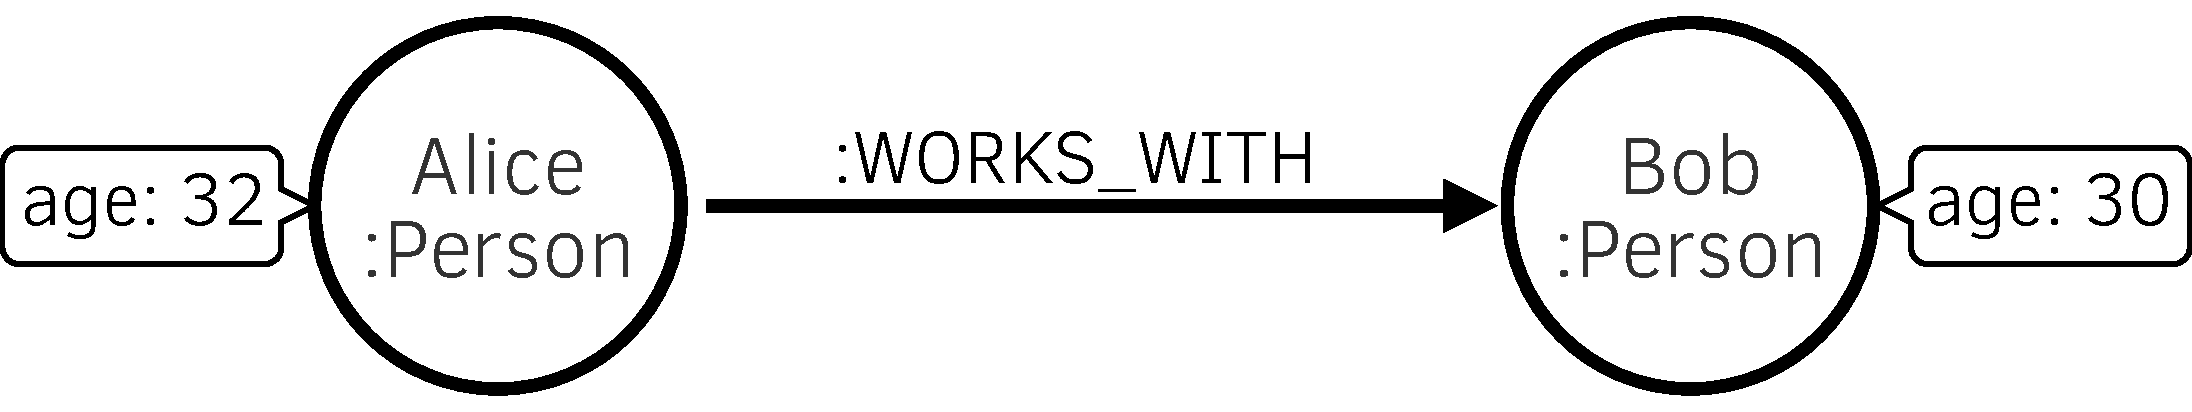
\includegraphics[width=0.6\textwidth]{graph-example}
	\caption{Typed and labeled property graph example.}
	\label{fig:graph-example}
\end{figure}


My approach utilizes typed (labeled) property graphs (see~\Cref{fig:graph-example}).

\subsubsection{Graph Computing Technologies}
The practice of data storage and processing is encumbered with space and time trade-off. This trade-off is also present in various graph computing technologies. This section discusses the categorization of these technologies and mentions a few technologies of which the most popular ones are detailed in~\cref{sect:graph-databases}.

The landscape of graph storing and processing solutions is populated and diverse (see~\cite{zhang_-memory_2015}). The basic categorization of software graph database solutions is the following. Graph computing technologies can be divided into two groups: 1)~on-line, real-time, and 2)~global analyzing, batch-processing graph databases. The former can be divided into in-memory, and persistent databases.

\paragraph{In-Memory Graph Toolkits}
The challenge of big data problems shed light on that the existing disk-based systems can not offer timely response due to the latency of hard disks. The role of storage shifted from the hard drive to the memory of the system. In-memory graph databases are constrained to graphs that fit into the main memory. Thus these systems are single-user systems that are oriented towards low-latency graph analysis.

The locality of data allows the usage of rich algorithm libraries and the choice of the adequate graph representation with respective space-time trade-off. The constraint of space allows large graphs (with millions of edges) to be stored and processed, but this may not be sufficient in all cases.

Example in-memory graph toolkits: \emph{Apache Giraph}\footnote{\small\url{http://giraph.apache.org}}, \emph{Microsoft Graph Engine}\footnote{\small\url{https://www.graphengine.io}} (formerly \emph{Trinity}), \emph{Apache Spark GraphX}\footnote{\small\url{http://spark.apache.org/graphx/}}, \emph{WhiteDB}\footnote{\small\url{http://whitedb.org}}.

\paragraph{Persistent, Real-Time Graph Databases}
Persistent graph databases are the prevalent group of graph computing technologies. Unlike in-memory graph tools, graph databases persist data on hard drives, thus are able to store billions of edges on a single machine and distributed systems can handle hundreds of billions of edges. These databases can provide multi-user concurrency, transactional semantics and eventual consistency.

Since global graph algorithms are not feasible, these systems are optimized for local neighborhood analysis and concurrent access. Global graph analytics are inefficient due to the communication overhead and the computational overhead, e.g., ensuring ACID transactional semantics.

Example for persistent, real-time graph databases: \emph{InfiniteGraph}\footnote{\small\url{http://www.objectivity.com/products/infinitegraph/}}, \emph{Neo4j} (see \cref{sect:neo4j}), \emph{OrientDB}\footnote{\small\url{http://orientdb.com}}, and \emph{Titan}~\cite{titan}.

\paragraph{Batch-Processing Graph Frameworks}
In case there is no real-time requirement for an analysis that accesses the whole dataset, batch-processing graph frameworks can be used for global analytics. Since there is also no requirement for quick response time, the applied algorithm can even scan data multiple times and leverage sequential reads from the disk. These systems can be used to periodically process data and feed back the results into real-time graph databases. Most of these frameworks utilize Hadoop for storage (HDFS) and processing algorithms implemented using the MapReduce paradigm.

Example batch-processing graph frameworks: \emph{Apache Hama}\footnote{\small\url{https://hama.apache.org}} and \emph{Apache Giraph}\footnote{\small\url{http://giraph.apache.org}}.

\subsection{Evaluating Queries on a Data Structure}
Numerous strategies exist for defining and executing queries over data structures. They can be defined in an imperative manner with programming languages like a navigation described in \emph{Gremlin}\footnote{\small\url{http://gremlin.tinkerpop.com}} over a graph database. Declarative solutions also exist, where the query plan is calculated from the query formalized in a declarative language (like \emph{SQL}\footnote{Structured Query Language}, \emph{SPARQL}\footnote{SPARQL Protocol and RDF Query Language}, and \emph{Cypher}) and execution is performed by a query framework (such as \emph{4store}\footnote{\small\url{https://github.com/garlik/4store}} and \emph{Neo4j}). Graph pattern matching -- one of the declarative querying solutions, supplemented by imperative logic -- forms the foundation of my approach.

\subsubsection{Graph Pattern Matching}
\textquote[\cite{csmr}]{Graph patterns are a declarative, graph-like formalism representing a condition (or constraint) to be matched against instance model graphs. The formalism is useful for various purposes in model-driven development, such as defining model transformation rules or defining general purpose model queries including model validation constraints. A graph pattern consists of structural constraints prescribing the interconnection between nodes and edges of a given type.

A match of a pattern is a tuple of pattern parameters that fulfill all the following conditions:
\begin{enumerate}[topsep=0pt]
	\item have the same structure as the pattern,
	\item satisfy all structural and attribute constraints,
	\item and does not satisfy any negative application condition (NAC) describing cases when the original pattern does not hold.
\end{enumerate}}

% TODO figure

\subsection{Graph Databases}
\label{sect:graph-databases}
Since my approach is based on graph-based data handling, it is essential to employ the most suitable technique. Related to my approach suitable refers to having the following traits: being fast, flexible, versatile, and easy to use and deploy. In this section I give an overview on the most promising candidates and justify why I have chosen Neo4j as the foundation of my approach.

\subsubsection{Neo4j}
\label{sect:neo4j}
Neo4j is the most popular~\cite{db-engines-ranking} and most mature NoSQL graph database, developed by \emph{Neo Technology}. It is open-source, well-documented and continuously-developed. Neo4j is available in two editions: a free \emph{Community Edition} and a paid \emph{Enterprise Edition}.~\cite{neo4j}

\paragraph{Architecture}
It can be deployed two ways: in \emph{server mode} the database is started separately and listens for queries on its HTTP REST and Bolt interface; where in \emph{embedded mode} it runs in the same JVM as the only client application.

\paragraph{Data Model}
The graph model of Neo4j is an implementation of a labeled property graph. The relations are labeled and the nodes can hold multiple labels; the nodes and relations can both hold properties.

\paragraph{Sharding}
Although the \emph{Enterprise Edition} of Neo4j has a high availability solution and supports clustered replication and cache sharding, it does not support sharded data storage over a cluster of devices. This results in the advantage of low latency (clustering provides scale out capabilities for read), the ability to handle transactions with ACID (Atomicity, Consistency, Isolation, and Durability) semantics.~\cite{neo4j-product}

\paragraph{Query Language}
Neo4j provides two methods for data queries out-of-the-box: an object-oriented native Java API for graph navigation and Cypher, a graph pattern description and query language with declarative and imperative traits. Additional interfaces may be loaded as a plugin, like the imperative Gremlin query interface~\cite{neo4j-gremlin-plugin}.

One of Cypher's best features is the readability of its syntax (see~\Cref{sect:division-by-zero} for examples). It provides an intuitive way to describe patterns of nodes and relations in the graph and also connections between subpatterns using bound identifiers for nodes and relations. Cypher also manages the indexes and constraints of the graph database. Negative application conditions (NAC) can be also expressed, describing constraints that should not hold for the matches.

Other interesting and useful features of Cypher include:
\begin{itemize}[topsep=0pt]
  \item Transitive closure over a set of edge labels, with optional repetition binding.

%        It is worth noting that an arbitrary sequence of edge labels can not be set as a repeating subpattern on its own, but temporary edges can be utilized to emulate this behavior.
  \item Java procedures can be stored in the server as a plug-in and called from inside the queries. This way an arbitrary logic with multiple queries can be stored on the Neo4j server and executed with a Cypher query. This can solve cases where it is not possible to express the query in Cypher; ranging from duplicating a node (with parameters and labels) to inferring the metamodel (from the nodes and relations already in the database).
  \item Parameterized queries may be utilized for faster evaluation.
%  \item List predicates evaluating predicates for all/any/none or single one nodes of the path.
%  \item Iterating and unwinding\footnote{transforming into rows} a collection in the query.
%  \item Finding the shortest path.
%  \item Mathematical functions.
%  \item Query profiling.
\end{itemize}

\subsubsection{Alternative Graph Databases}
Although other database solutions, like Titan~\cite{titan} or OrientDB might serve as an alternative, the rapid development and feature set of Neo4j ruled them out as a candidate for my approach.

For rapidly changing, albeit smaller datasets, incremental querying using VIATRA~\cite{viatra} Query over EMF~\cite{EMF} models can be a solution. Since VIATRA stores the database in-memory, it is not suitable for my approach.


\section{Integrated Development Environment (IDE)}
\label{sect:IDE}
Apart from the continuous integration workflow, static analysis tools are usually employed by developers within the integrated development environment they use. In this section I introduce one of the many freely available IDEs, and detail how static analysis tools can be integrated with it.

\subsection{Visual Studio Code}
\label{sect:visual-studio-code}
Visual Studio Code~\cite{vscode} is Microsoft's take on a lightweight, yet powerful Integrated Developer Environment for modern programming languages. It is available for free for Windows, macOS and Linux. It comes with built-in support for JavaScript, TypeScript and has a growing ecosystem of extensions for other languages, theming, and developer support~\cite{vscode-extensions}.

Debugging is also made easy, as the editor can be attached to the running code and the developer can add break points, look at call stacks and evaluate statements with an interactive console. With the relatively small package, Git support comes built-in: reviewing changed lines, staging files, making commits can be made right in the IDE.

\subsubsection{IntelliSense}
Visual Studio Code's syntax highlighting and autocomplete system is called IntelliSense, that also provides better completion based on variable types, function definitions, and imported modules. IntelliSense provides syntactical features like \emph{format on type}, \emph{outlining}; and also language service features like \emph{peek}, \emph{go to definition}, \emph{find all references} and \emph{rename symbol}.

To make these smarter functions possible, JavaScript service relies upon the TypeScript language service to handle JavaScript source code. It uses the same type inference system as TypeScript to determine the type of a value. (It recognizes the \emph{``ES3-style''} class declaration.) Explicit JSDoc annotations can also be used, in case the type inference does not provide the desired type information. For major libraries it is also possible to download an import a type definition file.

\subsubsection{Extensions}
Visual Studio Code is built with extensions in mind. Extensions make it possible to add new languages, themes, debuggers, and to connect to additional services. The framework runs them in a separate process, ensuring they will not slow the editor down.

Every extension uses the same model to describe its contribution (how it is registered in the framework), activation (when it is loaded) and the same way to access the VS Code extension API. There are two special type of extensions: language servers and debuggers, which have their own additional protocols.

Extensions are the building blocks of VS Code. When activated, every extension runs in a shared host process, separate from the IDE. This ensures that the IDE itself can remain responsive even if an extension is resource-heavy or not well-written.

An extension is a package of source code, resources, and configuration files. They have support for:
\begin{itemize}[topsep=0pt]
  \item Activation -- it is possible to specify when an extension is loaded: when a specific file type exists in the workspace or is opened; or when a command (described in the configuration) is executed via the \emph{Command Palette} or the key combination.
  \item Editor -- the extension can read and manipulate the editor's content.
  \item Workspace -- the extension can access working files, modify the content of the status bar and show information messages (and more).
  \item Eventing -- it is also possible to subscribe and react to the life-cycle events of the editor such as: open, close, change events of the editor (and more).
  \item Evolved editing -- rich language support can be provided, including IntelliSense services, peek, hover and diagnostic (info, warning and error messages).
\end{itemize}

\paragraph{Language Servers} The language server framework and its sample implementation helps developers create a dedicated process for resource-heavy language server applications. It is the better design choice if the extension may slow down other extensions while working. Its possibilities are limited, as custom communication between the client extension and the language server needs modification in the underlying communication protocol handler.

\paragraph{Debuggers} Connecting an external debugger written for any language to VS Code is also possible through the VS Code Debug protocol.

\subsection{Alternative IDEs}
There are several alternatives to Visual Studio Code. \emph{Atom}\footnote{\small\url{https://atom.io}}, \emph{Eclipse}\footnote{\small\url{https://eclipse.org}}, and \emph{WebStorm}\footnote{\small\url{https://www.jetbrains.com/webstorm/}} can all be extended with a plugin adding extra features for a given language. Since VSC is one of the most actively developed lightweight IDEs aiming for JavaScript (and TypeScript) development, I have developed an extension integrating the IDE with my framework (see~\Cref{sect:ide-integration}).

% !TEX root = ../main.tex
\chapter{Related Work}
\label{chap:related-work}

In this chapter I enumerate a subset of similar systems, approaches and discuss related work.

\section{Tern}
\textquote[http://ternjs.net]{Tern is a stand-alone code-analysis engine for JavaScript. It is intended to be used with a code editor plugin to enhance the editor's support for intelligent JavaScript editing. Features provided are:

\begin{itemize}[topsep=0pt]
	\item Autocompletion on variables and properties
	\item Function argument hints
	\item Querying the type of an expression
	\item Finding the definition of something
	\item Automatic refactoring
\end{itemize}

Tern is open-source (MIT license), written in JavaScript, and capable of running both on node.js and in the browser.}

The Tern suite is a modular, extendable stand-alone system. Editor plugins communicate with the Tern server module, connected to the Acorn parser (introduced in~\Cref{sect:acorn}) and the inference engine. Third-party plugins can introduce implementation environmental or behavioral information for the system, for example ECMAScript module loading rules, or node.js~\cite{nodejs} specific variables.~\cite{tern-docs}


\section{TAJS}
Type Analyzer for JavaScript (TAJS)~\cite{tajs} is a dataflow analysis tool infering type information and call graphs. The current version (as of 2016) can model scripts of ECMAScript 3; it also contains model of the standard library and partial model of the HTML DOM and browser API.~\cite{tajs-git}

The initial aim of TAJS was to warn programmers for the following problematic cases. This enumeration follows~\cite{jensen_type_2009}.

\begin{itemize}[topsep=0pt]
  \item invoking a non-function value as a function
  \item reading an absent variable
  \item accessing a property of \code{null} or \code{undefined}
  \item reading an absent property of an object
  \item writing to variables or object properties that are never read
  \item implicitly converting a primitive value to an object
  \item implicitly converting \code{undefined} to a number
  \item calling a function object both as a function and as a constructor or passing function parameters with varying types
  \item calling a built-in function with an invalid number of parameters or with a parameter of an unexpected type
\end{itemize}


\section{TRICORDER}
TRICORDER~\cite{tricorder} is a pluggable program analysis platform used internally at Google, helping developers and reviewers notice possible problems with code changes. The system mainly supports C$++$, Go, and Java codes, but it has support for JavaScript too.

Related researches show that static analysis tools are either not used or ignored, when not configured correctly and take more time from the user than necessary. \textquote[\cite{tricorder}]{High false positive rates, confusing output, and poor integration into the developers' workflow all contribute to the lack of use in everyday development activities \cite{johnson2013don, layman2007toward}.

TRICORDER introduces an effective place to show warnings. Given that all developers at Google use code review tools before submitting changes, TRICORDER's primary use is to provide analysis results at code review time. This has the added benefit of enabling peer accountability, where the reviewer will see if the author chose to ignore analysis results.}


\section{JavaScript Parsers}
\label{sect:javascript-parsers}
In this section I showcase the most used, \emph{trending} JavaScript parser technologies and justify why I have chosen the Shape Security Shift family as the parser and additional toolset for my approach.

\subsection{Acorn}
\label{sect:acorn}
Acorn~\cite{acorn} is an open-source, small JavaScript written in ES6. It is up-to-date, able to parse ECMAScript version 3, 5, 6, 7, and the newest one, 8. The resulting AST structure of the parser conforms the ESTree specification~\cite{estree}.

It is also able to parse multiple files into a single AST, connected with a \code{Program} node. This is not to be confused with an ASG connecting multiple ASTs. To analyze and navigate in the resulting AST, Acorn provides a walker interface, to be used with a visitor pattern based algorithm.

The parser is also configurable with several options, \code{locations} being one of the most useful for my approach. Setting this option stores the location of the represented source snippet in the AST node. There is also an error-tolerant version of the parser enabling parsing unfinished or syntactically incorrect sources.

\textquote[\cite{acorn}]{Acorn is designed support allow plugins which, within reasonable bounds, redefine the way the parser works. Plugins can add new token types and new tokenizer contexts (if necessary), and extend methods in the parser object.}

\subsection{Esprima}
Esprima is also an open-source, ECMAScript standard-compliant parser. It fully supports ES7, and produces ESTree models. It has a great user-base and several tools depend on it. It also has experimental support for JSX, an XML syntax extending JavaScript for React~\cite{react}, \textquote[\cite{react-tutorial}]{a declarative, efficient, and flexible JavaScript library for building user interfaces}.


\subsection{Shift}
\label{sect:shift}
The Shift~\cite{shift} family consists of several tools. Besides the parser, there is a scope analyzer, a code validator, fuzzer, and a code generator, besides others.

\subsubsection{Shift AST}
The reason behind the number of tooling in this family is due to the fact that Shift does not conform the ESTree specification. In 2014, Shape Security, the company behind Shift announced a new JavaScript AST specification~\cite{shift-spec}. This specification was developed with ECMAScript 6 in mind, along with analysis and transformation.

The specification describes interface for an AST syntax that can represent the structure of an ECMAScript source code. According to Shape Security, a \textquote[\cite{shift-spec-comparison}]{good AST format…

\begin{itemize}
	\item minimizes the number of inhabitants that do not represent a program.
	\item is at least partially homogenous to allow for a simple and efficient visitor.
	\item does not impede moving, copying, or replacing subtrees.
	\item discourages duplication in code that operates on it.
\end{itemize}
}

\subsubsection{Shift Scope Analyzer}
\textquote[\cite{shift-scope}]{The Shift Scope Analyser produces a data structure called a scope tree that represents all of the scoping information of a given program. Each element of the scope tree represents a single scope in the analysed program, and contains many pieces of information, including:

\begin{itemize}[topsep=0pt]
	\item the scope type (there are 12 of them!)
	\item the AST node associated with the scope
	\item variables declared within that scope, each of which points to its declarations and references
	\item whether the scope contains a with statement or direct call to eval, making it dynamic
\end{itemize}}

\subsubsection{Additional Notes}
\begin{itemize}[topsep=0pt]
	\item Besides JavaScript, most of the Shift family is also available for Java projects. This makes it easier to integrate it with projects and tools only available for Java.

	\item Shape Security has a project, Bandolier~\cite{bandolier} for packaging projects with ES6 modules into a single JavaScript file, imitating the export-import mechanism, related to my approach.

	\item Shape Security is also developing a semantic transformer~\cite{shift-semantics-java} for ECMAScript ASTs, also related to my approach.
\end{itemize}

\subsection{Comparison of Parser Technologies}
In order to find a best parser and related technologies, I had to compare them: measure their speed, investigate their parameters and output model, and transform their extra functions into potential features of my approach.

\subsubsection{Speed} Although speed is not the most important property of a system aiming to make sure no errors are present, swift response can boost the performance of the user. \Cref{table:speed-comparison-of-parsers} shows the time difference between parsers processing various source codes repositories. The benchmark~\footnote{\url{http://esprima.org/test/compare.html}} was run on a personal computer without specific considerations or fine-tuning for benchmarks. Its sole purpose is to get a rough comparison between the different technologies available.

It is visible that Shift NEE\footnote{Early error checking disabled. NEE -- No Early Errors} is one of the fastest parsers available.

\begin{table}[!htb]
\centering
\begin{tabular}{@{}lllllll@{}}
\toprule
\textbf{Source}                                               & \textbf{\begin{tabular}[c]{@{}l@{}}Esprima\\ 2.7.2\end{tabular}} & \textbf{UglifyJS2}                                      & \textbf{Traceur}                                        & \textbf{\begin{tabular}[c]{@{}l@{}}Acorn\\ 2.4.0\end{tabular}} & \textbf{Shift}                                          & \textbf{\begin{tabular}[c]{@{}l@{}}Shift\\ (NEE)\end{tabular}} \\ \midrule
\begin{tabular}[c]{@{}l@{}}jQuery.Mobile\\ 1.4.2\end{tabular} & \begin{tabular}[c]{@{}l@{}}154.0\\ ±22.3\%\end{tabular}          & \begin{tabular}[c]{@{}l@{}}244.6\\ ±8.4\%\end{tabular}  & \begin{tabular}[c]{@{}l@{}}304.6\\ ±15.1\%\end{tabular} & \begin{tabular}[c]{@{}l@{}}215.3\\ ±16.9\%\end{tabular}        & \begin{tabular}[c]{@{}l@{}}480.7\\ ±13.1\%\end{tabular} & \begin{tabular}[c]{@{}l@{}}119.9\\ ±11.9\%\end{tabular}                    \\
\begin{tabular}[c]{@{}l@{}}Angular\\ 1.2.5\end{tabular}       & \begin{tabular}[c]{@{}l@{}}125.5\\ ±16.3\%\end{tabular}          & \begin{tabular}[c]{@{}l@{}}212.2\\ ±11.2\%\end{tabular} & \begin{tabular}[c]{@{}l@{}}254.1\\ ±20.7\%\end{tabular} & \begin{tabular}[c]{@{}l@{}}146.3\\ ±18.6\%\end{tabular}        & \begin{tabular}[c]{@{}l@{}}452.7\\ ±12.5\%\end{tabular} & \begin{tabular}[c]{@{}l@{}}94.6\\ ±18.2\%\end{tabular}                     \\
\begin{tabular}[c]{@{}l@{}}React\\ 0.13.3\end{tabular}        & \begin{tabular}[c]{@{}l@{}}134.7\\ ±10.8\%\end{tabular}          & \begin{tabular}[c]{@{}l@{}}221.6\\ ±8.9\%\end{tabular}  & \begin{tabular}[c]{@{}l@{}}258.5\\ ±13.4\%\end{tabular} & \begin{tabular}[c]{@{}l@{}}176.9\\ ±15.6\%\end{tabular}        & \begin{tabular}[c]{@{}l@{}}496.4\\ ±11.6\%\end{tabular} & \begin{tabular}[c]{@{}l@{}}116.1\\ ±14.2\%\end{tabular}                    \\ \midrule

\textbf{Total}                                                & \textbf{414.3 ms}                                                & \textbf{678.4 ms}                                       & \textbf{817.2 ms}                                       & \textbf{538.5 ms}                                              & \textbf{1429.8 ms}                                      & \textbf{330.6 ms}                                                          \\ \bottomrule
\end{tabular}

\caption{Speed comparison of JavaScript parsers.}
\label{table:speed-comparison-of-parsers}
\end{table}

\subsubsection{Metamodel and Precision}
For analysis and transformation purposes it is rather important to have a model with as much and as precise information as possible. If the parser produces a model conforming a detailed metamodel, it is easier to differentiate seemingly similar cases.

Based on the comparison~\cite{shift-spec-comparison} between the ESTree and the Shift AST specification, it is visible that Shift is a better choice if more detail is required.

% \subsubsection{Development Activity}
% \subsubsection{Platforms Supported}

% !TEX root = ../main.tex
\chapter{Overview of the Approach}
\label{chap:overview-of-the-approach}

In this chapter I introduce the high-level architecture overview of the proposed framework. The chapter also discusses each component in detail including details on how they cooperate.

\section{Architecture}
\label{sect:architecture}
\Cref{fig:architecture-overview} shows the overview of the framework's architecture. Since the novelty of the approach is how the source code representation is handled --- stored, transformed, and queried --- the heart of the approach is visualized on the right half of the figure. This is embedded and utilized in the framework itself, and integrated into the continuous integration circle and user-facing systems.

\begin{figure}[!htb]
  \centering
  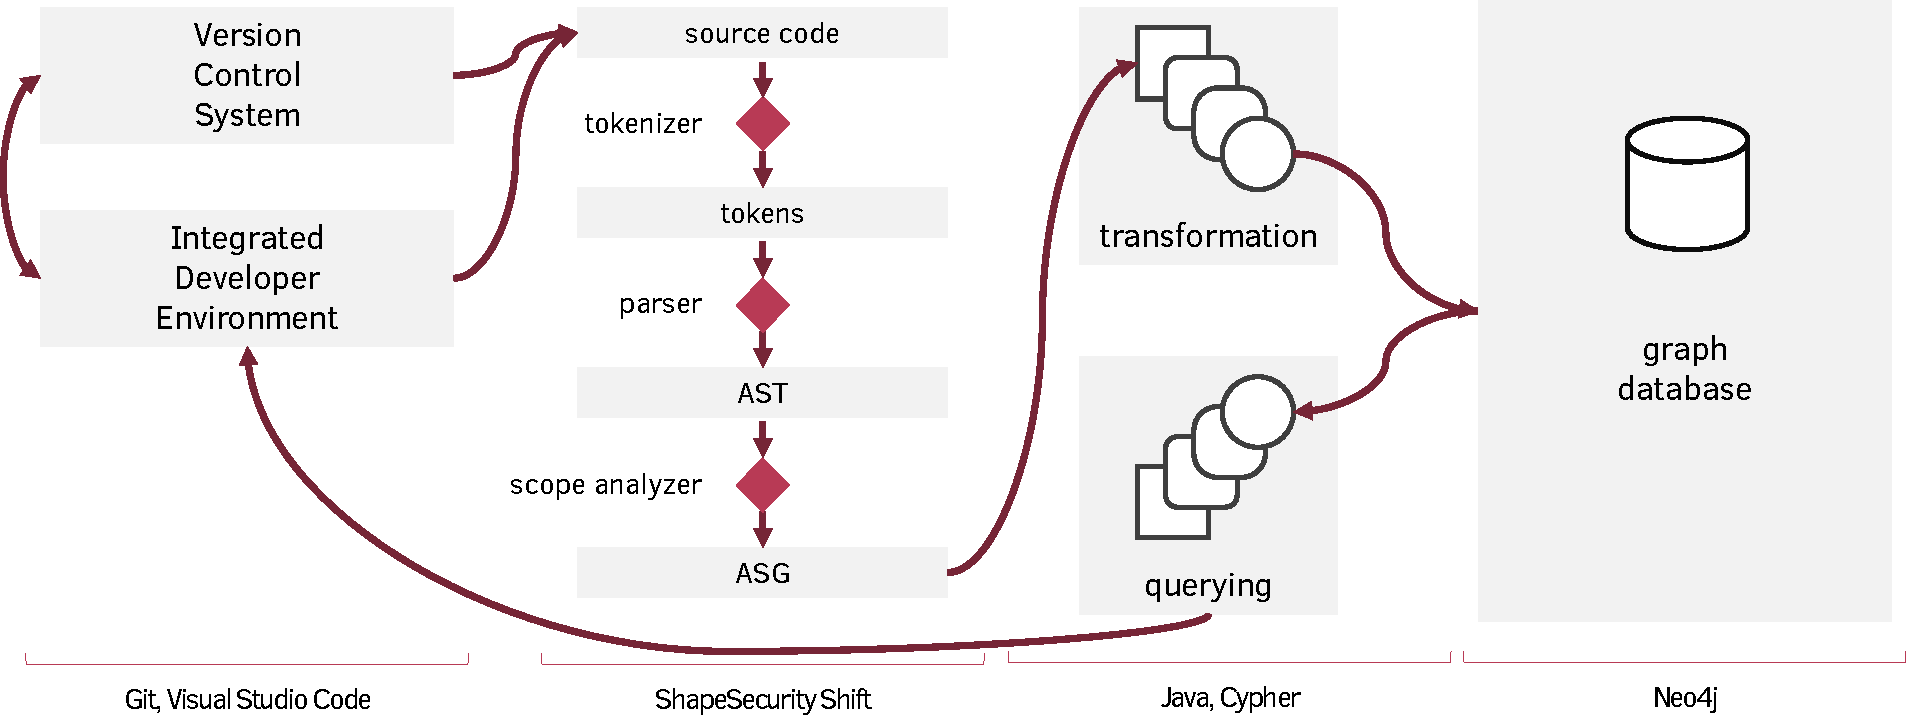
\includegraphics[width=\textwidth]{architecture-PPT.pdf}
  \caption{Architecture overview of the approach.}
  \label{fig:architecture-overview}
\end{figure}
% TODO update
% TODO add edge labels


\section{Main Components}
% TODO intro text (maybe the difference between this, steps of processing and the enumeration)

\subsection{Workflow Integration Points}
The framework is intended to be integrated with at least two types of development tooling. First, connecting to the \emph{Version Control System} makes it possible to extend the continuous integration workflow and provide the users of the system with current information about the codebase they are working on. Second, connecting to the \emph{Integrated Development Environment} empowers their users with feedback on the current modifications.

\subsubsection{Version Control System (VCS)}
Version control systems are change management systems for files (e.g., documents, software code). They store revisions of the current set of files managed by the system. Each revision is differentiated with a timestamp and also the person performing the changes are associated with a revision.

Version control is one of the most essential collaboration tools. When developers work on the same codebase, especially when the codebase is large, they need to share the code and work on it at the same time. Using a VCS, one can investigate the current version of the codebase at a selected revision. Also, it is possible to determine the changes performed between two revisions, manage multiple development branches with the same root and merge the changes made in these.

Integrating a VCS into the architecture makes it possible to extend the workflow with the features of the framework. By automatically calculating the changeset and forwarding this information to the framework, it is possible to keep an up-to-date representation of the version controlled data source.

The most known implementations are Git~\cite{git}, Subversion (SVN)~\cite{svn}, Mercurial (Hg)~\cite{hg}.

\subsubsection{Integrated Development Environment (IDE)}
An IDE is an application for (software) developers that integrates several tools making it easier to write, compile, and test the product. Integrated development environments are detailed in \Cref{sect:IDE}.

In the architectural overview, the IDE also represents the working set of the software and its dependencies available on the developer's computer. This working set also contains the developer's modifications that are not yet transferred to the shared VCS.
% TODO clarify, rephrase


\subsection{Transforming the Source Code}
\label{sect:overview-transforming-the-source-code}
One of the most important third party components of the approach is the source code parser. This component is used to transform a given source file, a \emph{compilation unit} into a model representation of the syntax and semantics of the source code. The process itself is detailed in~\Cref{sect:source-code-processing}.

A source code parsing toolkit with the following traits makes it possible to integrate it into the framework with ease:

\begin{itemize}[topsep=0pt]
  \item Provide the Abstract Syntax Tree and Abstract Semantic Graph for the parsed source file.

  \item Also provide scoping information
  % TODO

  \item Source code position
  % TODO

  \item Metamodel for the representation
  The more detailed metamodel, the better.
\end{itemize}

Since the \emph{Shape Security Shift} toolkit (detailed in~\Cref{sect:shift}) suits these requirements well, I have used the Java implementation of the \emph{Shift Parser}, and \emph{Scope Analyzer}.


\subsection{Graph Maintenance}
The novelty of my approach is how it processes, stores and connects the source code representation in a graph database. In this section I'll discuss how the subgraphs of the source code files are prepared and then connected to each other constructing a connected graph representing the whole source code repository.

The process can be summarized in 4 concise sentences:
\begin{enumerate}[topsep=0pt]
  \item The repository is transformed one file-by-file.
  \item The ASG \emph{model} is transformed into a \emph{property graph}.
  \item After every file is processed, the ASG subgraphs are interconnected using graph transformations.
  \item In case a file is added/modified/deleted, the corresponding subgraph is also added/removed and reprocessed/removed from the graph.
\end{enumerate}

This process and the algorithm for graph maintenance is detailed in~\Cref{sect:maintaining-the-graph}.


\section{Steps of Processing}
The following enumeration presents the basic algorithm for processing, transforming, storing and analyzing the source code repository.

\subsection{Initial State}
The graph representation of the repository follows the development of the source code. Thus initially both the graph database and the repository are empty. When the database is initialized, metadata and initial database structure can be inserted, so the queries executed later can build on the existence of this structure.

\subsection{Calculating the Changes to Propagate}
Once there are modifications published in the repository or the IDE, it is the integrating tool's responsibility to notify the framework. This can be an event hook for the IDE or the CVS, for example. The changes to a file at a given path may be the following:

\begin{itemize}[topsep=0pt]
  \item \emph{Addition.} In case a new file is added, it is processed, and the subgraph representation is stored in the database.

  \item \emph{Modification.} Since the approach is incremental with a file-level granularity, the modification of a file's contents requires the removal of the whole old and addition of the new subgraph.

  \item \emph{Removal.} The removal of a file causes the removal of the subgraph too.
\end{itemize}

\subsection{Maintaining the Graph}
\label{sect:maintaining-the-graph}

The file changes are processed one-by-one. The integrating tool notifies the framework, specifying the path and content of the file along with additional metadata. The content is then preprocessed using the parser resulting in a model representation.

\subsubsection{Transforming the Instance Model}
This representation of the parser conforms the metamodel based on the syntax and semantics of the source language. But the property graph database can not import the data in this form, thus it needs to be transformed. \Cref{fig:object-to-graph} presents the transformation of a Java object structure into a graph based on the basic rules detailed in this section.

\begin{figure}[!htb]
  \centering
  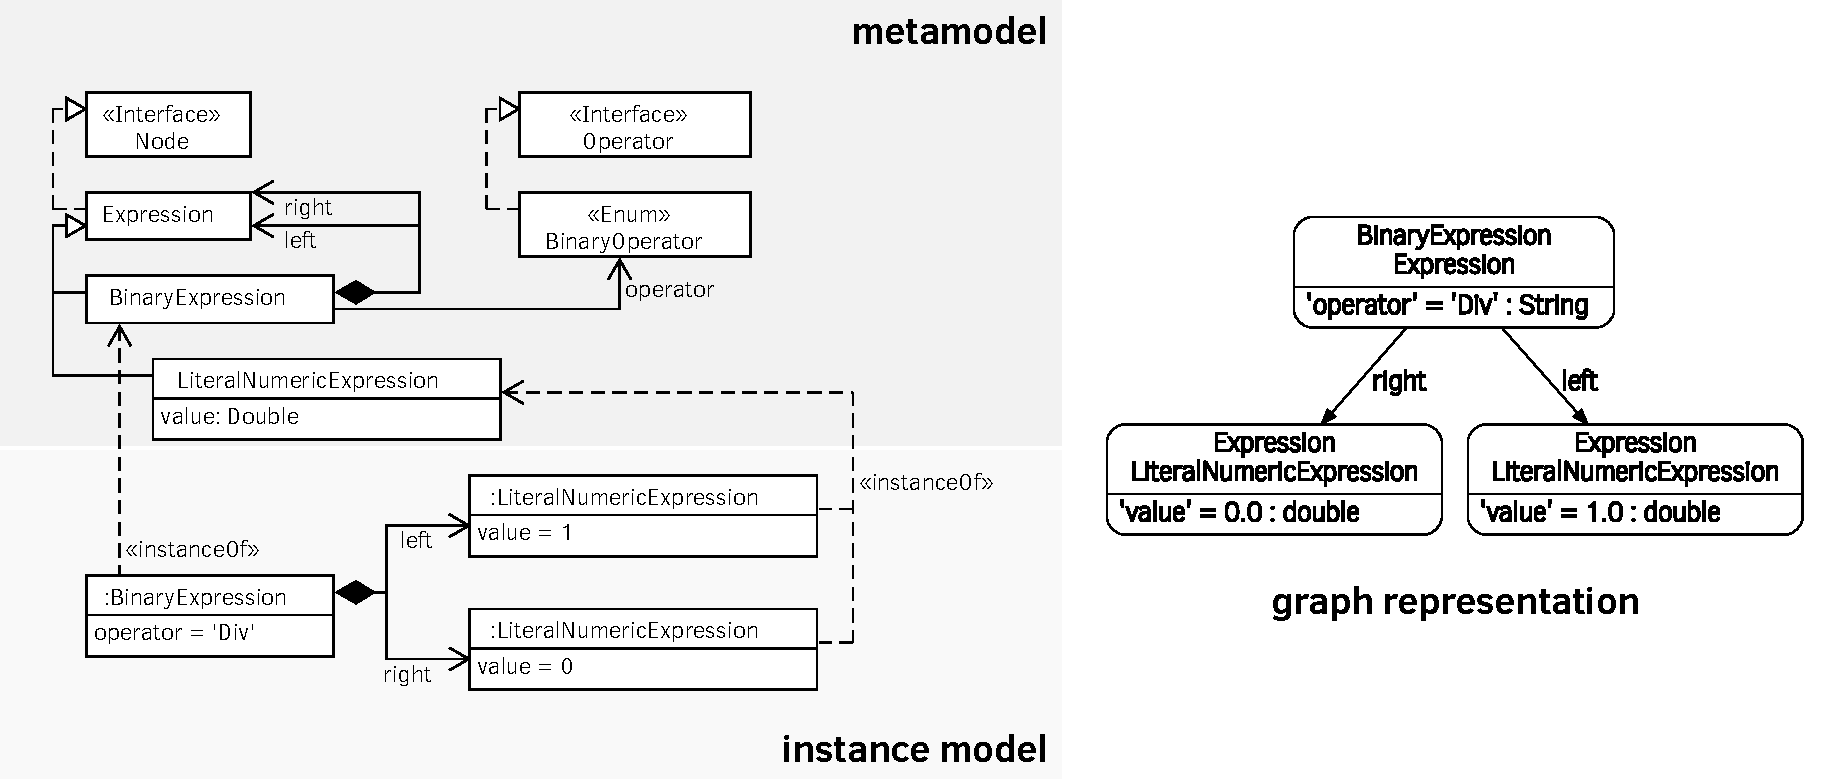
\includegraphics[width=\textwidth]{object-to-graph.pdf}
  \caption{Transformation of a Java object structure into a graph.}
  \label{fig:object-to-graph}
\end{figure}

In order to acquire information from this model and transform it, one either knows its metamodel and iterates over every element or --- if the programming language of the parser allows --- uses reflection. In my approach I use the combination of the Shift parser written in Java --- thus using the reflective approach --- and the Neo4j labeled property graph database.

\paragraph{Typed Nodes}
Every AST or ASG node is a node in the graph. The graph node is typed with the class, superclasses and interfaces of the represented model entity.

% CFG end node is also created for every node

\paragraph{Node Properties}
Every property of a model entity --- regardless of whether they are its own or inherited from its supertypes --- are also transferred to the graph node. These properties are also stored with their basic type: \emph{double}, \emph{string} or \emph{boolean}.

\paragraph{Labeled Relations}
References in the model are represented in the graph as relations, directed edges. The relations are labeled after the name of the references.

\paragraph{Collections}
The metamodel also contains several reference collections: maps, lists and tables. Maps and tables are represented in the graph as a new node, with appropriately labeled relations to the referred nodes.

Lists are transformed similarly. In order not to lose ordinal information, the items are related to the referrer with two routes (see~\Cref{fig:graph-list}).

\begin{figure}[!htb]
  \centering
  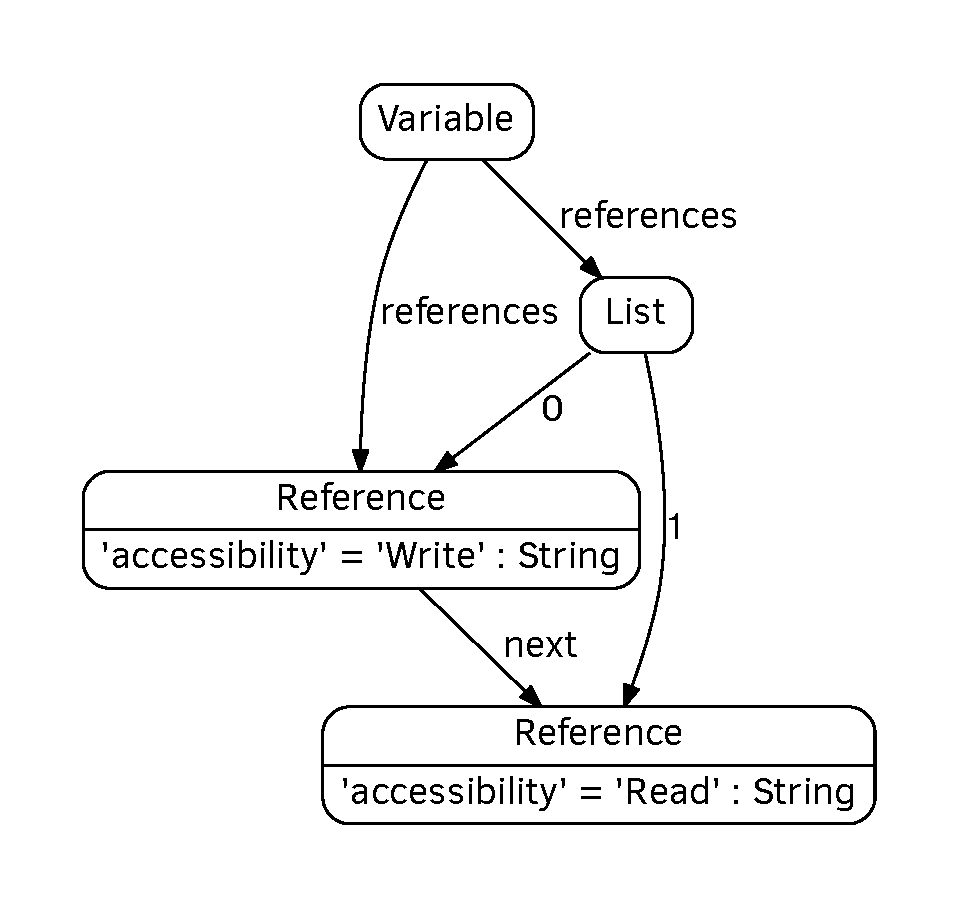
\includegraphics[width=0.5\textwidth]{graph-list.pdf}
  \caption{Graph Representation of a List}
  \label{fig:graph-list}
\end{figure}

The first route is direct; the referrer has a relation to every item of the list (labeled with the name of the list). The second route has an additional \emph{List} node between the two, and its relations are labeled with the index of the item. The sequential items also have a direct, chaining relation.

% last item of the list is marked
%\paragraph{Functional Elements}

\paragraph{Source Code Location}
To be able to report precise location for a problem, the graph also contains line and character information for the beginning and the end of every model entity.


\subsubsection{Storing the Graph Representation}
If the parser successfully processes the source code, the resulting ASG is transformed with the forementioned rules. In a writing transaction, the transformed graph is serialized and stored in the database.

\paragraph{Metadata}
Besides the ASG, additional properties are stored. For example, for every source file, a node exists in the graph connected to nodes belonging to the particular ASG. This makes it easier to handle nodes of a file as a whole.

\paragraph{Multilayered Graph}
With more complex rules it is also feasible to store multiple versions of the same file in the database. This makes it possible to maintain multilayered versioning for multiple users.

If the VCS supports branching the code development, the framework could also accomodate this behaviour. For example if two developers work on the \emph{master} development branch in their own IDE, there could be layers for each of them.

\begin{figure}[!htb]
  \centering
  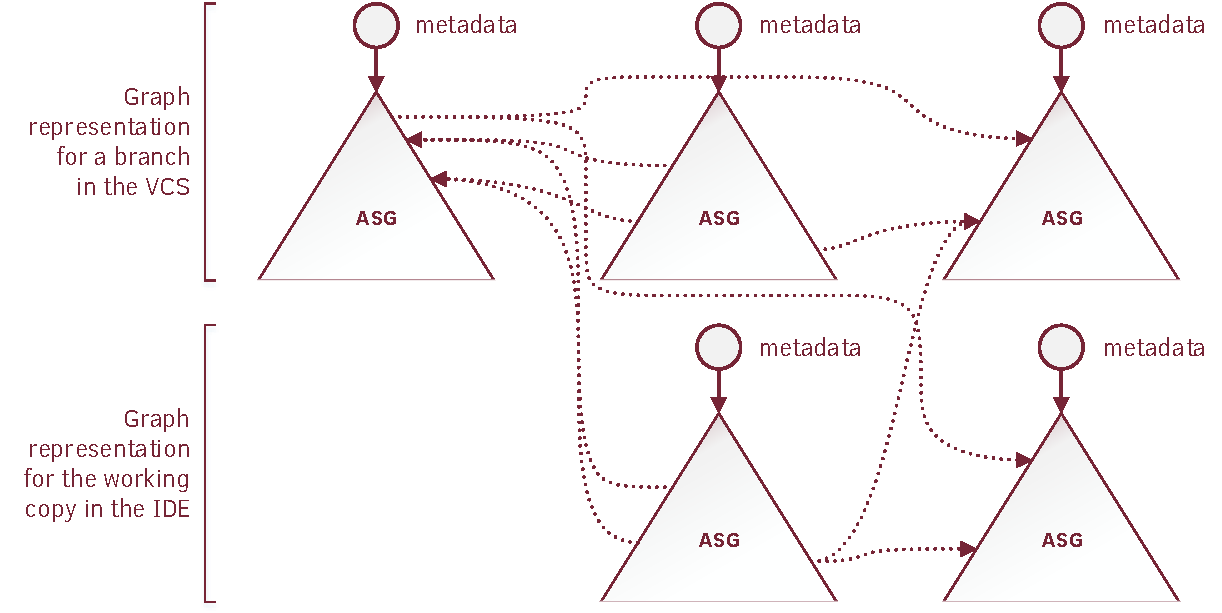
\includegraphics[width=\textwidth]{multilayer.pdf}
  \caption{Multilayered graph.}
  \label{fig:multilayered-graph}
\end{figure}

One layer containing every ASG for the \emph{master} branch. One layer for each user containing only the ASGs of their modified files. In these layers the ASGs are connected (based on the import and export statements) in the same layer, if both are present in the same. If not, they are connected to the corresponding file in the \emph{master} branch (see~\Cref{fig:multilayered-graph}).

\subsubsection{Transforming the Graph}
After the data has been stored in the database, it can be freely transformed with framework- or user-defined rules. This step may be utilized for transforming the set of subgraphs into one connected graph based on the export and import rules of the language.

Neo4j makes it possible to execute in-place transformations, where querying with pattern matching and manipulations may be declared in the same query. The possibilities of Neo4j are detailed in~\Cref{sect:neo4j}. Transformation examples are presented and visualized in~\Cref{chap:elaboration-of-the-workflow}.

\subsection{Executing Graph Queries}
By utilizing the built-in pattern-matching abilities of Neo4j, it is easier and more user-friendly to write pseudo-graphic, declarative patterns to find a structure in the graph --- compared to the generally used visitor patterns.~\cite{csmr} An example graph pattern query is detailed in~\Cref{sect:division-by-zero}.

If Cypher, the query language of Neo4j is not powerful enough to describe a constraint, one may also use arbitrary Java code. This code may be used inside the query or even command multiple queries and aggregate the result.

% !TEX root = ../main.tex
\chapter{Elaboration of the Workflow}
\label{chap:elaboration-of-the-workflow}

In this chapter I demonstrate the various steps of the static analysis workflow in detail. I employ small working source code examples in order to demonstrate the steps of the source code transformation. A prototype implementation of the proposed workflow is available as an open-source project at {\small\url{https://github.com/FTSRG/codemodel-rifle}}.

\section{Transforming the Source Code Into an AST}
As mentioned in~\Cref{sect:overview-transforming-the-source-code}, this transformation is carried out by the Shape Security Shift toolkit. The source code is passed to the parser along with the parameters for the parsing algorithm. Considering the new constructs introduced in ES6 (\Cref{sect:ecmascript}), I've chosen to parse every file as a \emph{Module}. This affects the grammar used in the parser and the resulting data model.
% TODO href Shift

The parse result of the one-line code snippet in~\Cref{lst:oneliner} was previously presented in~\Cref{fig:ast-asg-example}.

\begin{figure}[!htb]
	\begin{minipage}{\textwidth}
		\lstinputlisting[
			language=JavaScript,
			captionpos=b,
			caption={Basic example source code.},
			label={lst:oneliner},
		]{include/sources/oneliner.js}
	\end{minipage}
\end{figure}

\section{Storing the ASG in the Graph Database}
Once the source code is parsed and the ASG is returned, the framework updates the stored graph representation. Since \Cref{sect:maintaining-the-graph} details how the Java Object structure is transformed into a graph, this section only describes the queries used for the maintenance.

When a new file is added to the repository, there is no need to prepare the database. A new metadata node is created with the name and path of the file, and optionally the session identifier of the IDE it has been created and sent in to the framework. The subgraph representing the ASG is then inserted in a database transaction.

The newly created metadata node acts as a subgraph selector, since it is connected to every node belonging to the file (of the given session). This makes it easy to remove the file upon the removal of the file it represents.

In case the file has been modified, the nodes connected to its metadata node are removed, then the new graph is inserted.


\section{Division by Zero}
\label{sect:division-by-zero}
As one of the most basic and easy-to-discover mistakes, division by zero should be reported to the developer. In the context of mathematics, division by zero is undefined for the real numbers. In JavaScript, it may result in \code{NaN} or \code{Infinity}.

Without dynamic testing or symbolic execution it is rather hard to find this kind of expression, since the right side of the division may come from a variable. On the other hand, finding the cases where the right side is a literal is trivial.

Taking a look at~\Cref{fig:AST-PPT}, the graph representation of the previous example, it is relatively easy to find the problematic nodes. A natural language definition of the problem would sound like this: ,,we are looking for binary expressions that have a literal zero on the right side''.

\begin{figure}[!htb]
  \centering
  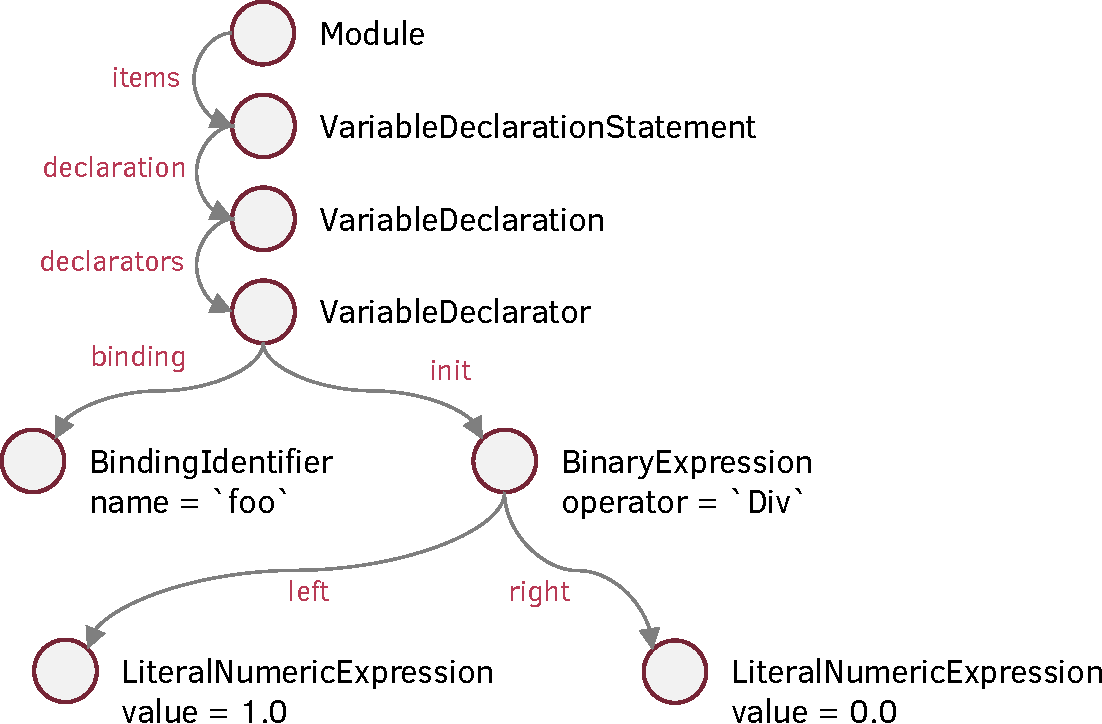
\includegraphics[width=0.8\textwidth]{AST-PPT.pdf}
  \caption{Graph representation of the code snippet of~\Cref{lst:oneliner}.}
  \label{fig:AST-PPT}
\end{figure}

One way to formalize this declarative definition in Cypher can be seen in~\Cref{lst:division-by-zero}. Executing this query on the AST of the source code would 1)~find matching nodes with the right type, 2)~bind them to the corresponding names, and 3)~check whether the required relations are present, resulting in a state like in~\Cref{fig:AST-query-PPT}. Finally, the result is the \code{BinaryExpression} node. By querying the source code location (also stored in the graph connected to the node) this query can report the precise location of the expression in the source code as problematic.

\begin{figure}[!htb]
	\begin{minipage}{\textwidth}
		\lstinputlisting[
			language=Cypher,
			captionpos=b,
			caption={Graph Pattern Matching Division by Zero.},
			label={lst:division-by-zero}
		]{include/sources/division-by-zero.cypher}
	\end{minipage}
\end{figure}

\begin{figure}[!htb]
  \centering
  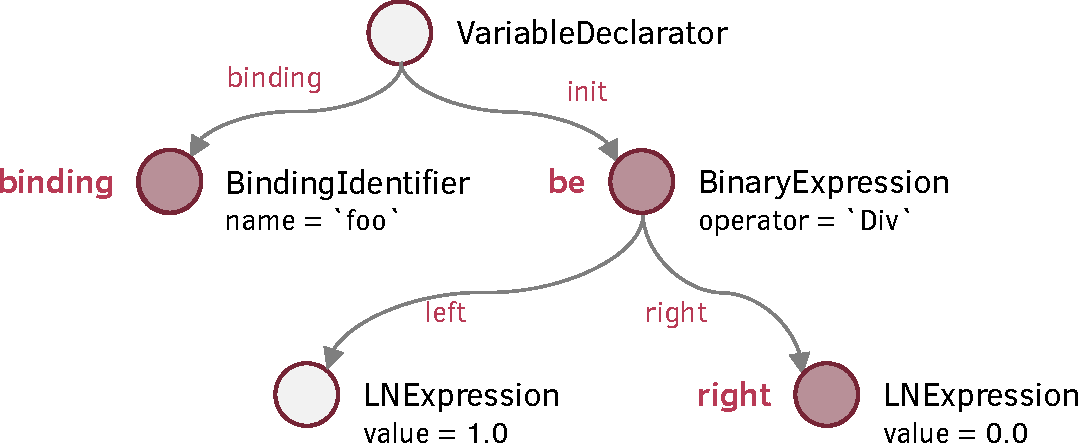
\includegraphics[width=0.8\textwidth]{AST-query-PPT.pdf}
  \caption{Graph representation of the query describing division by zero.}
  \label{fig:AST-query-PPT}
\end{figure}


\section{Handling Import and Export}
\label{sect:handling-import-export}
Since the beginning, JavaScript projects have grown tremendously. With the size of the average project, the language has also matured for handling bigger, more complex code repositories. With ES6, a module syntax has been introduced to spread the codebase into files, even directories. (Even before ES6 there have been several module systems, but ES6 described a standard for it.)

As described previously, I instruct the parser to process source files as modules. An ES6 \emph{module} differs in two ways from a \emph{script}: it is automatically interpreted as a \emph{strict-mode code}, and one can use \code{import} and \code{export} statements in them.

This section follows~\cite{ES6InDepth,ES6import,ES6export} and collects the most important details about the specifications.


\subsection{Export}
Everything declared inside a module belongs to the scope of the module. In order to let other modules to access them, they need to be explicitly exported.

\Cref{lst:es6-export} lists the various ways declaring a feature export. Just to list a few combinations; one may, for example, export expressions, variables, function and generator declaration statements either named, or using an alias. Or have default export expressions, even in an export statement.

\begin{figure}[htbp]
	\begin{minipage}{\textwidth}
		\lstinputlisting[
			language=JavaScript,
			captionpos=b,
			caption={ES6 export statement examples from MDN.},
			label={lst:es6-export},
		]{include/sources/es6-export-mdn.js}
	\end{minipage}
\end{figure}

Parsing these export statements result in different representation in the instance model and the resulting graph. \Cref{fig:es6-export-example} shows an example inline default export statement for a function named \code{foo}: \code{export default function foo() \{\}}. Note that the export statements are listed in the \code{Module}, but not in any of the \code{Scope}s.

\begin{figure}[htbp]
  \centering
  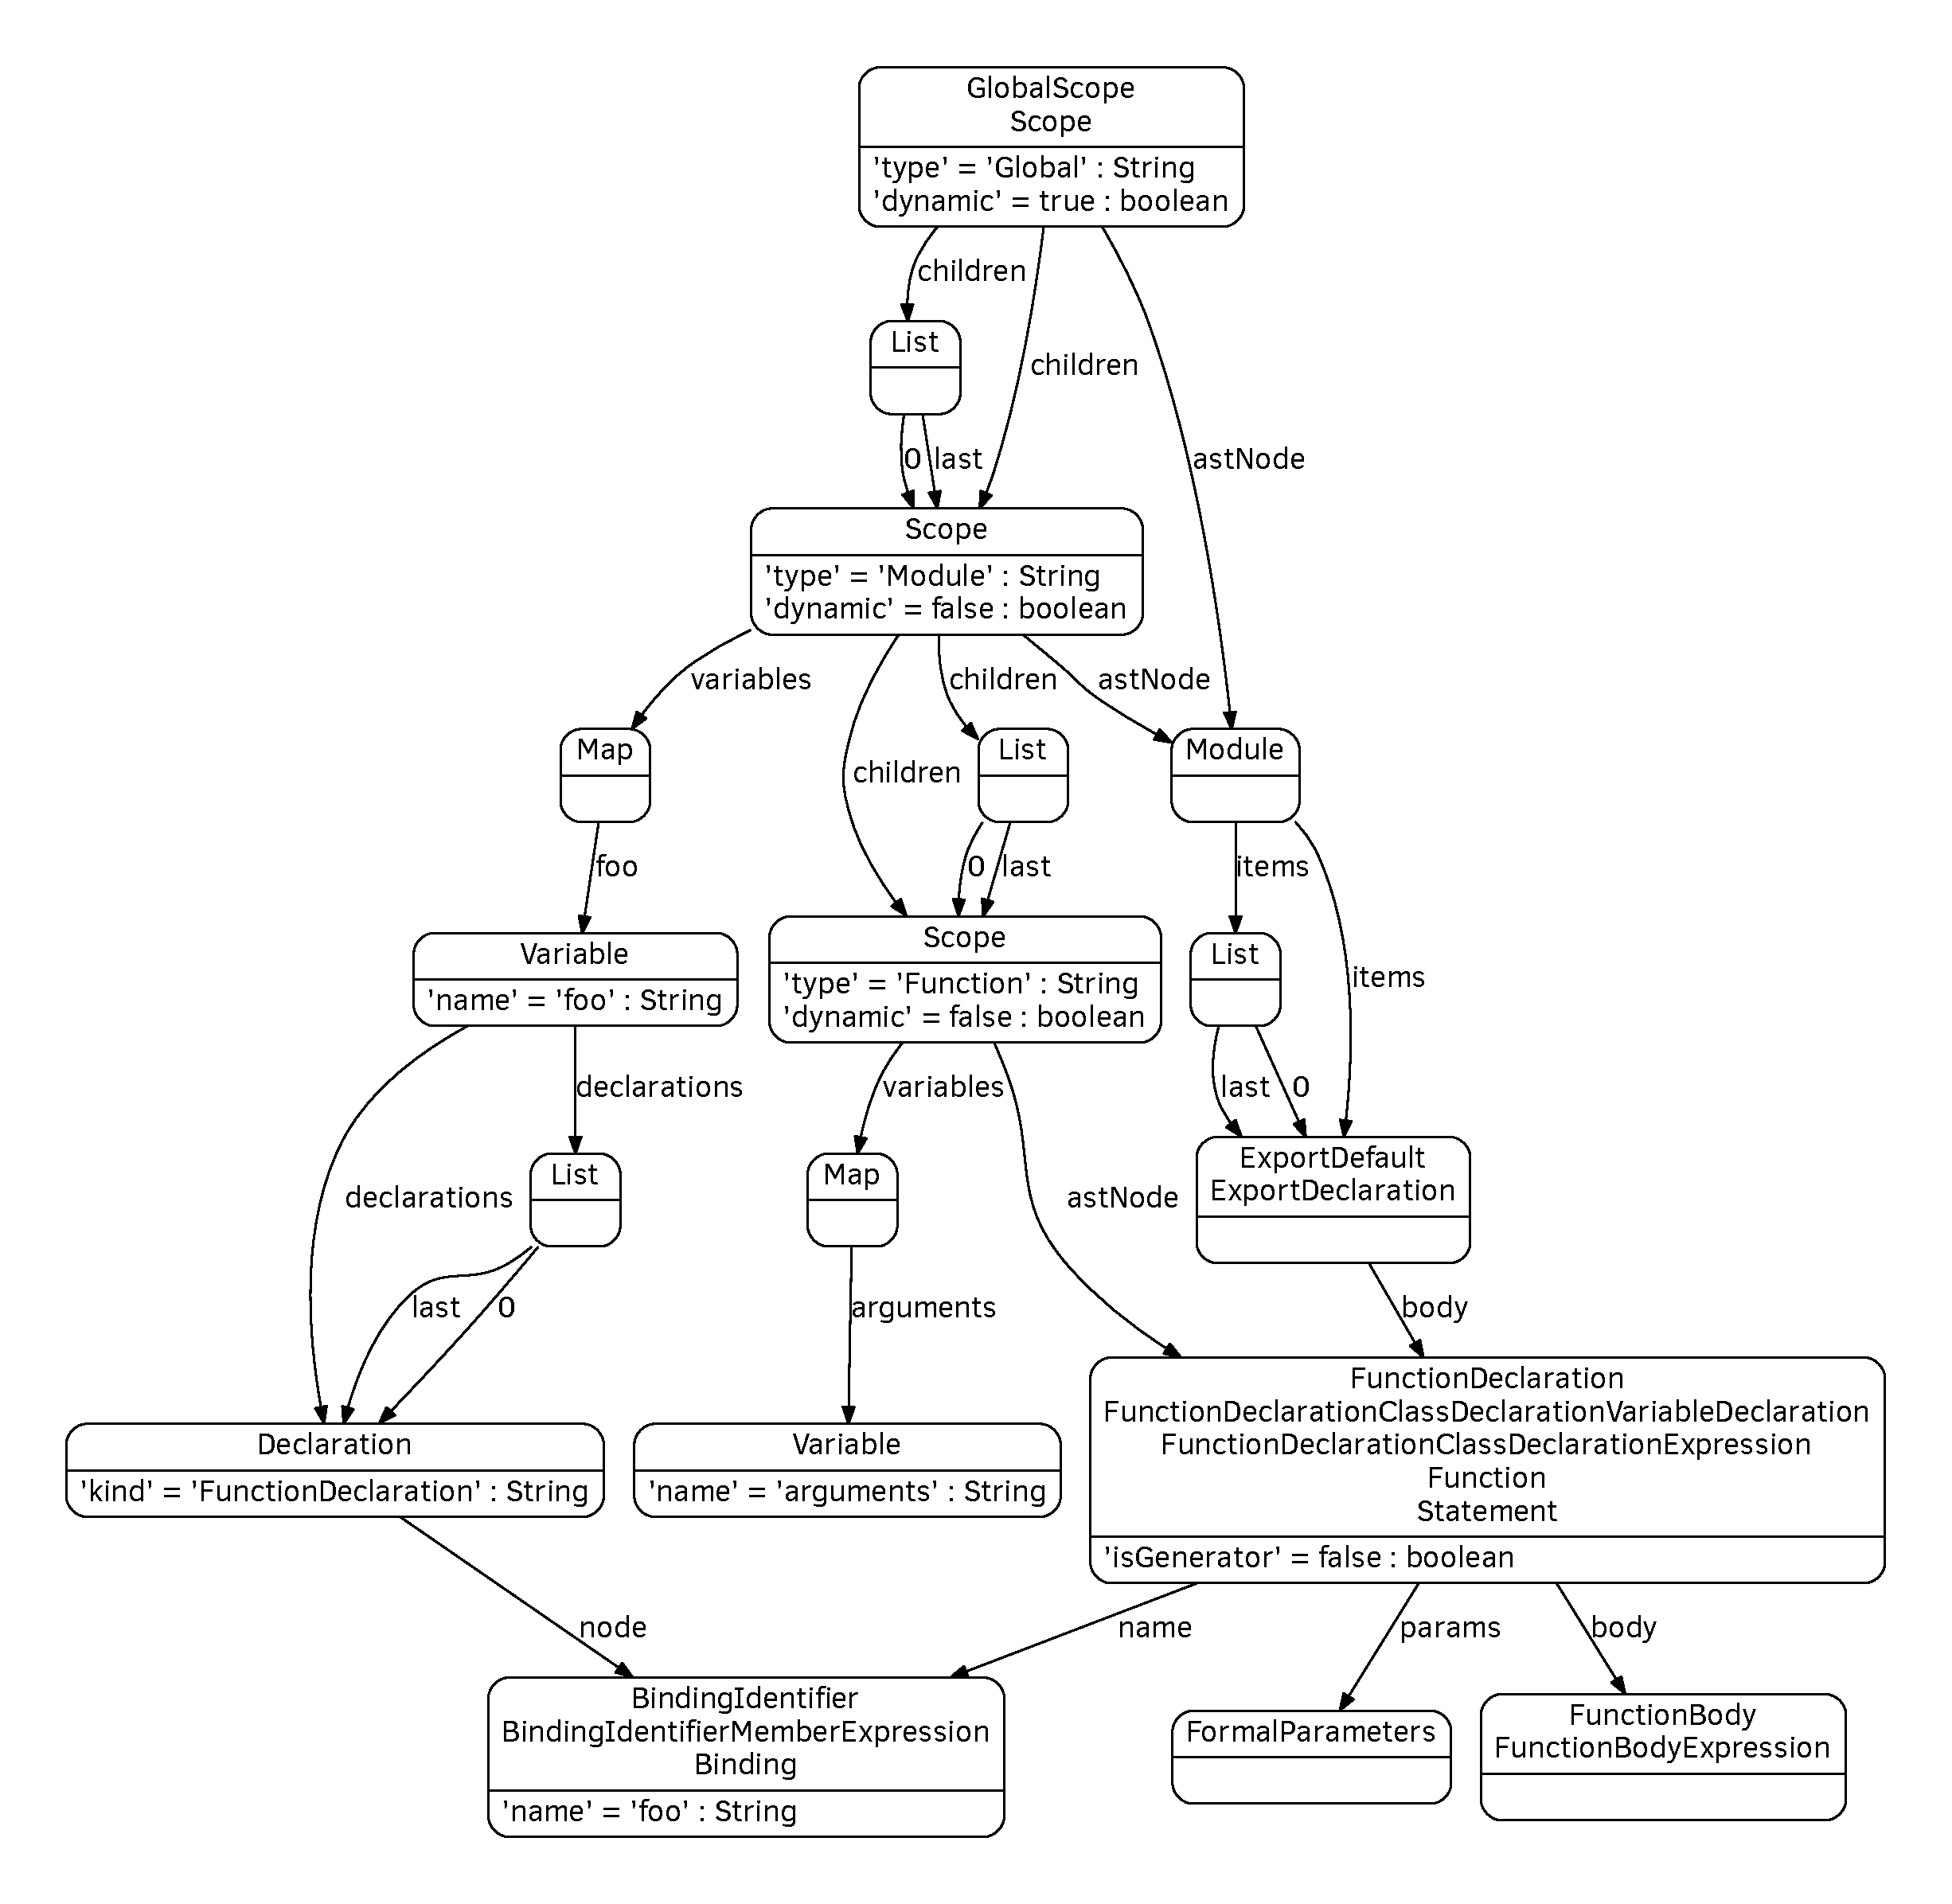
\includegraphics[width=\textwidth]{export-example}
  \caption{ES6 export statement example.}
  \label{fig:es6-export-example}
\end{figure}


\subsection{Import}
Like there are many ways for exporting features in a module, there are also several ways for importing them. \Cref{lst:es6-import} lists these.

\begin{figure}[htbp]
	\begin{minipage}{\textwidth}
		\lstinputlisting[
			language=JavaScript,
			captionpos=b,
			caption={ES6 import statement examples from MDN.},
			label={lst:es6-import},
		]{include/sources/es6-import-mdn.js}
	\end{minipage}
\end{figure}

The imported features are placed in the module-level global scope as a \code{Variable} without their declaring node, and the import statements are also present in the AST. \Cref{fig:es6-import-example} shows the ASG of a module importing and then using a function declaration (exported in the previous module): \code{import foo from "export"; foo();}.

\begin{figure}[htbp]
  \centering
  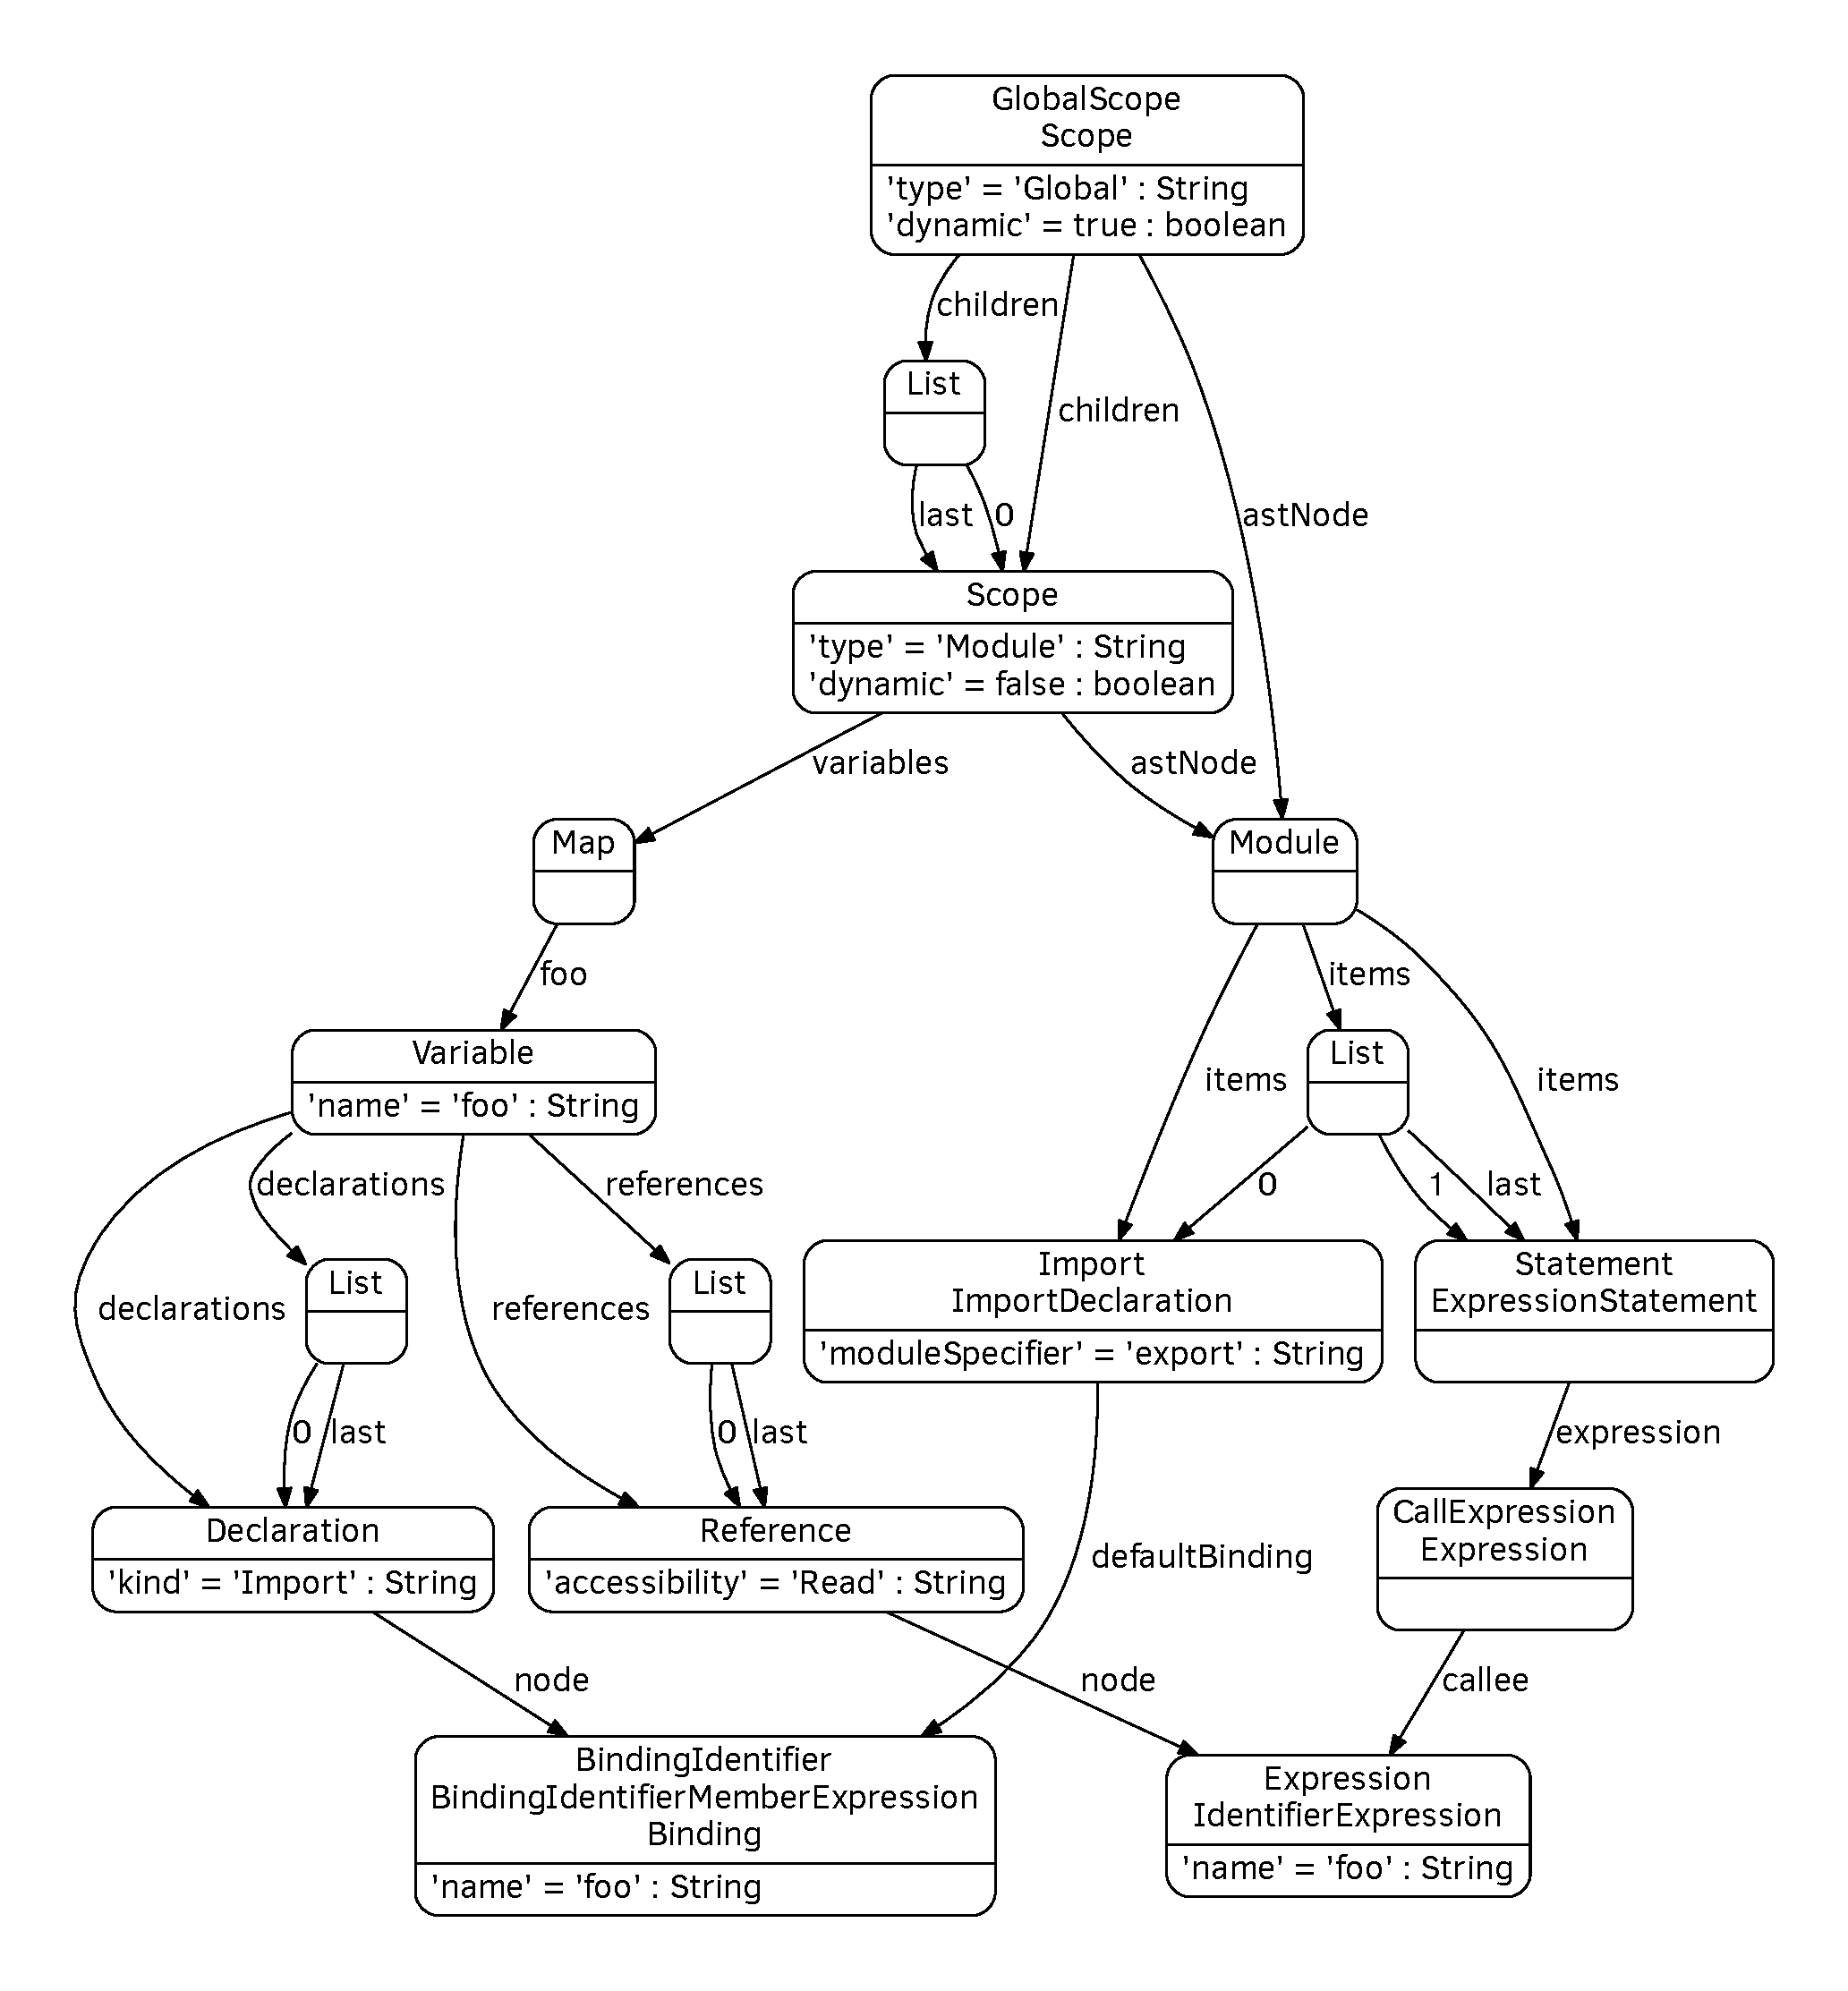
\includegraphics[width=\textwidth]{import-example}
  \caption{ES6 import statement example.}
  \label{fig:es6-import-example}
\end{figure}

\subsection{Connecting Imports to Exports}
Since there are several ways to both export and import features, there are even more combinations. This report does not aim to cover all of these, but to show that it is possible to connect graph module representations based on simple rules.

Executing the following steps emulates the resolution made by the interpreter of the source codes and connects the usages of the imported feature to the declaration of the exported one:

\begin{enumerate}[topsep=0pt]
	\item Find the imported \code{IdentifierExpression} in the \code{items} list of the \code{GlobalScope} node.
	\item Find the connected upstream \code{Variable} node.
	\item Find the \code{Declaration} for the \code{Export} that has a \code{Node} with the same \code{BindingIdentifier} as the import.
	\item Connect the \code{Variable} on the import side to the \code{Declaration} on the export side with a \code{declarations} relation.
\end{enumerate}

The Cypher query in~\Cref{lst:connect-import-export} manages to connect the exact type of imports and exports mentioned previously. Note that this query does not search for a file exporting the statement. For the correct match it should also check the metadata, whether the found node was declared in a file with matching absolute path.
% TODO absolute path

\begin{figure}[!htb]
	\begin{minipage}{\textwidth}
		\lstinputlisting[
			language=Cypher,
			captionpos=b,
			caption={Cypher query for connecting import and export statements.},
			label={lst:connect-import-export}
		]{include/sources/connect-import-export.cypher}
	\end{minipage}
\end{figure}

After executing the query in~\Cref{lst:connect-import-export}, the two ASG subgraphs are connected with a new edge (see~\Cref{fig:import-export-example}). This enables executing global-level queries addressing multiple modules. These newly added relations are always removed when either the source or the destination is removed, in case a module is modified. Thus it is optimal to run this query only when all of the files are already processed and the chance of modification in the near future is low. (This might happen after a modification is sent to the VCS or the developer saves the files in the IDE.)

\begin{sidewaysfigure}[htbp]
  \centering
  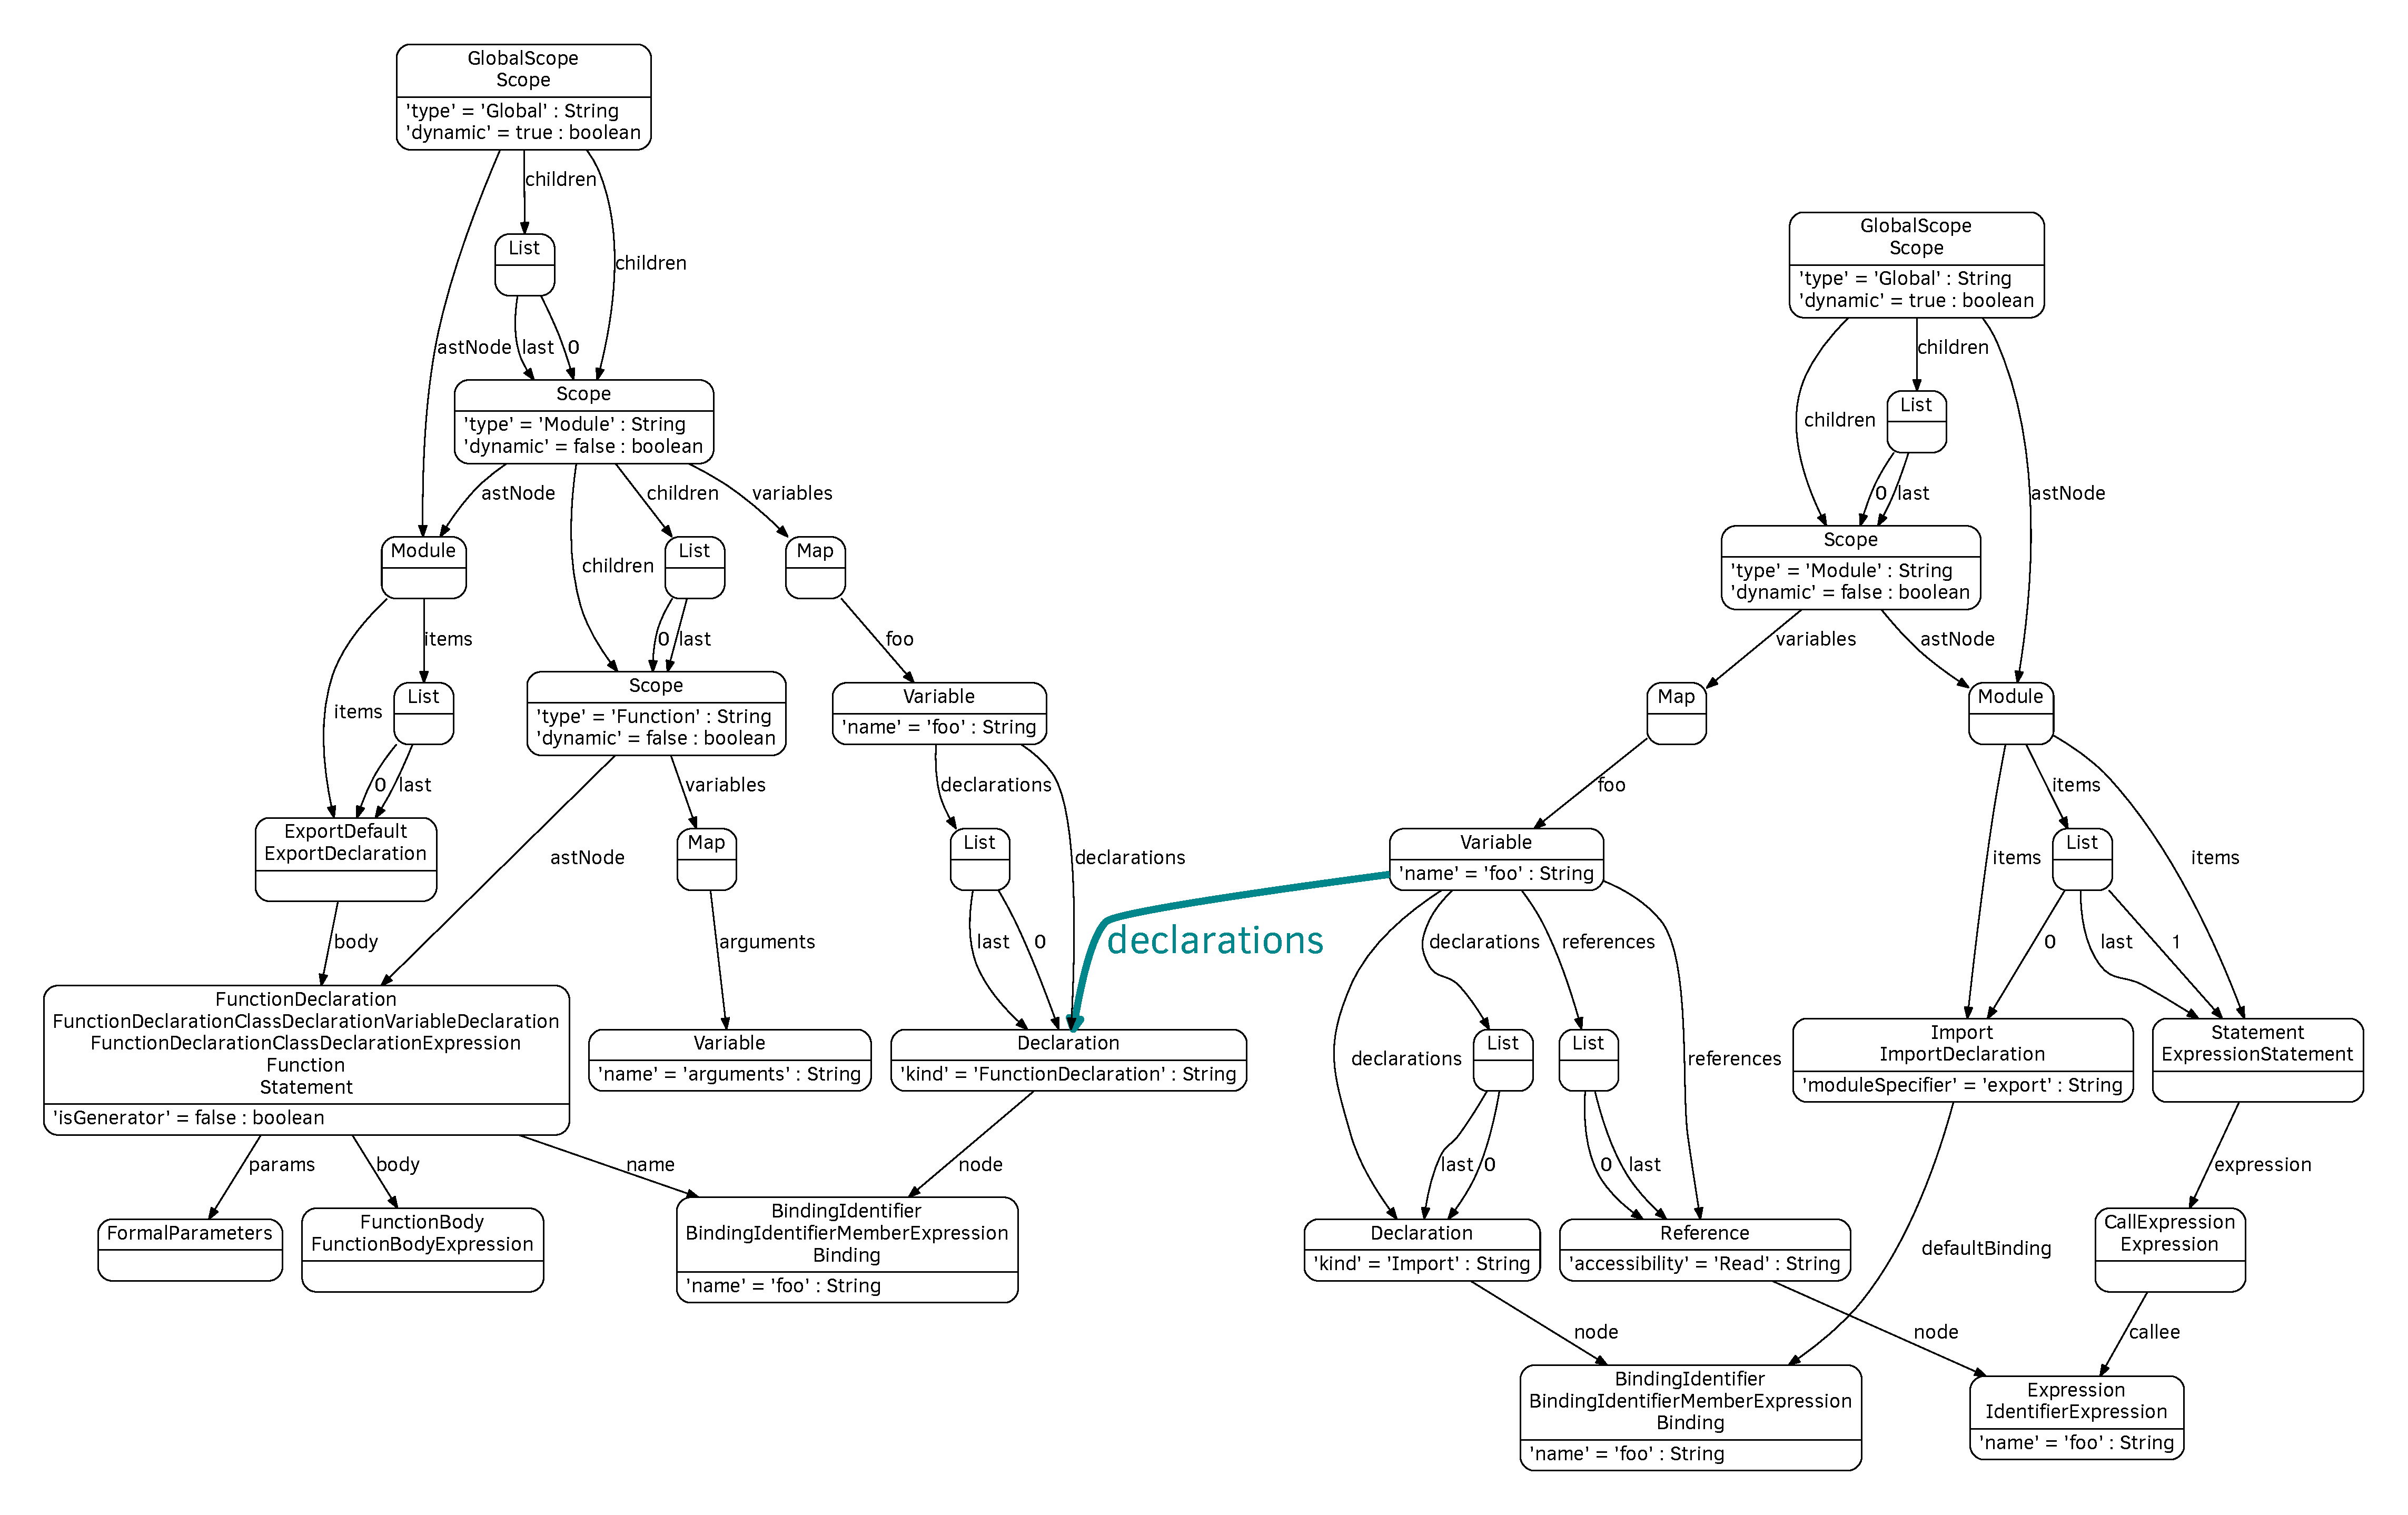
\includegraphics[width=\textwidth]{import-export-example}
  \caption{Connected ASG subgraphs.}
  \label{fig:import-export-example}
\end{sidewaysfigure}


\section{Dead Code Search}
\label{sect:dead-code-search}
Code that is written, but not used in the whole codebase is often called \emph{dead code}. Without symbolic execution it is a complex problem to decide what part of the code is reachable, but (excluding dynamic evaluation, e.g., \code{eval} in JavaScript) it is feasible to find function declarations in a file which are possibly not referenced in the local scope.
% TODO cite

\subsection{Search Algorithm as a Graph Query}
If a function declaration is not exported from the module and no exported declaration references it, it is highly likely that the declaration is unreachable and contains \emph{dead code}. With the following steps and the Cypher query described in~\Cref{lst:dead-code} it is possible to locate dead code in a file.

\begin{enumerate}
	\item Find the called \code{FunctionDeclaration}s target for every \code{CallExpression}.
	\item Find every call from the body of a function.
	\item Create a \code{calls} relationship between the caller and the callee \code{FunctionDeclaration}.
	\item Find the exported \code{FunctionDeclaration}s that can be entrance points.
	\item Find every \code{FunctionDeclaration} that should be available through the entrance points.
	\item Return every \code{FunctionDeclaration} that are not in this list.
\end{enumerate}

\begin{figure}[!htb]
	\begin{minipage}{\textwidth}
		\lstinputlisting[
			language=Cypher,
			captionpos=b,
			caption={Cypher queries for finding dead code.},
			label={lst:dead-code}
		]{include/sources/dead-code-search.cypher}
	\end{minipage}
\end{figure}

\subsection{Evaluating the Result}
For the sake of conciseness, I present the query for a simplified version of this algorithm, which only works with a single module in the database.

Compared to other commercially available software, this solution is able to detect more dead code scenarios: e.g., circular references without incoming calls (see~\Cref{fig:dead-code-result}. Instead of reporting the problems one-by-one or layer-by-layer, it reports the clique, without user input.

\begin{figure}[htbp]
  \centering
  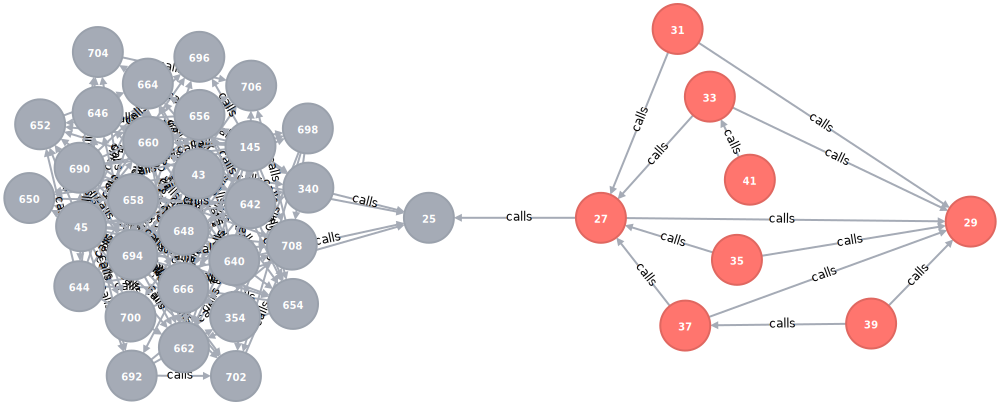
\includegraphics[width=\textwidth]{dead-code-result}
  \caption{Call graph with self-referencing clique in red.}
  \label{fig:dead-code-result}
\end{figure}
% TODO recolor and replace caption

\subsection{Transformation in a Transaction}
This query utilizes several possibilities only available in Neo4j. Since the query modifies the database, but the modifications are derived information, they should not be stored in the database. Database transactions that can be discarded, but still query the modified database are highly utilized here.

It is not possible to declare transitive closure\footnote{Transitive closure is marked with an asterisk in Cypher.} over arbitrary node type and edge label sequence in one Cypher query. This can be tackled by utilizing the \emph{trick} of starting a new transaction, writing the database and immediately querying the modified created data, then discarding the transaction. One can match and replace every sequence with a new, dedicated labeled edge and declare a transitive closure over it, but this requires the database to be modified (see~\Cref{fig:transitive-closure}).

\begin{figure}[htbp]
  \centering
  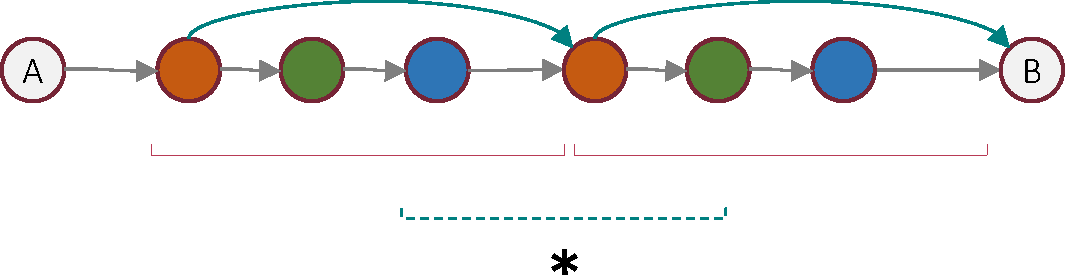
\includegraphics[width=\textwidth]{transitive-closure}
  \caption{Transitive closure over arbitrary node type and edge label sequence.}
  \label{fig:transitive-closure}
\end{figure}


\section{Control Flow Graph (CFG)}
Control Flow Graphs (CFG) are graph representations of the computation and control flows in the program. In this graph the nodes represent statements that are not interrupted by control changes. Directed edges represent possible flow of control between the two nodes. Nodes can have multiple incoming and outgoing edges.~\cite{IntroductionToCompilers}
\Cref{fig:CFG-PPT} presents an example CFG.

\begin{figure}[htbp]
  \centering
  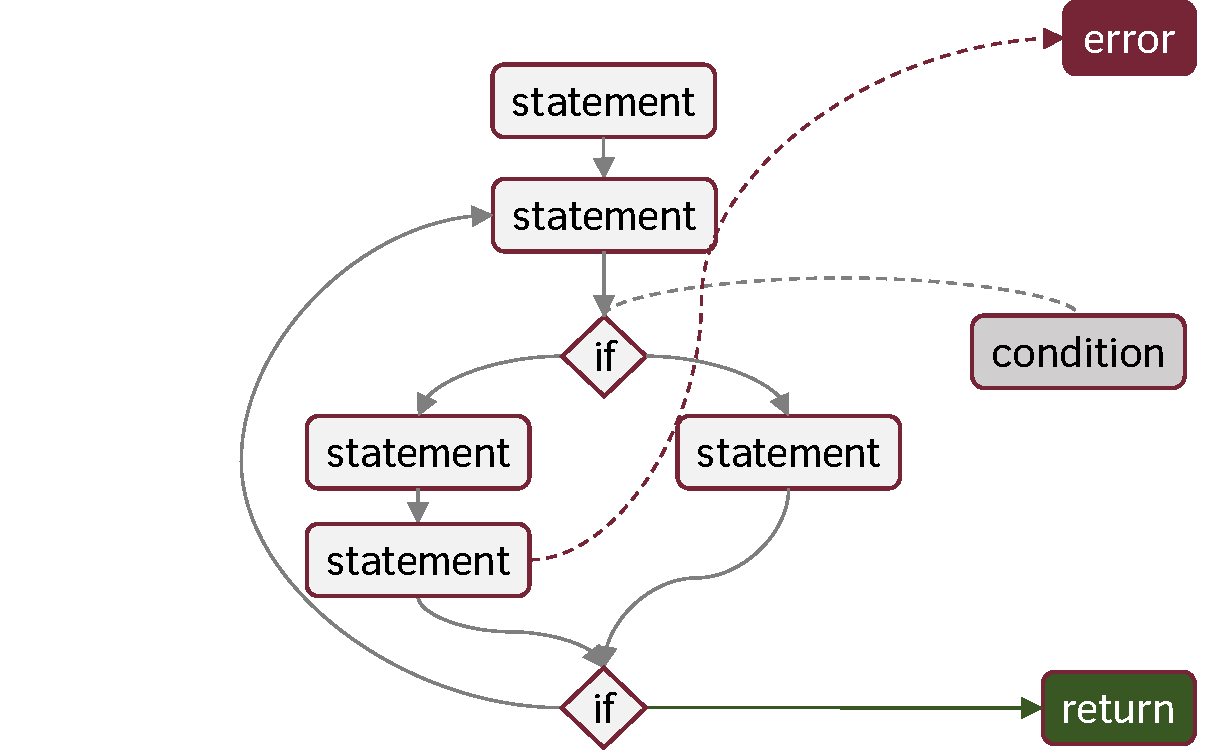
\includegraphics[width=0.75\textwidth]{CFG-PPT}
  \caption{Example control flow graph.}
  \label{fig:CFG-PPT}
\end{figure}
% TODO fix the CFG (if before return)

In this section I demonstrate how to transform the basic ASG structures into a CFG, and to utilize the result for static analysis.

\subsection{Theoretically Possible Paths}
\label{sect:cfg-paths}
As previously mentioned, nodes can have multiple incoming and outgoing edges. At execution time when the state of the program is at a given CFG node --- based on the dynamic state of the execution --- it may continue with any statement of the corresponding subsequent nodes.

Without running or interpreting the source code it is only possible to find and map every scenario in the ASG and transform them into nodes and edges in the CFG. A possible execution path is a path in the graph from one of the entry nodes to one of the exit nodes. The constraints on this path may be unsatisfiable, thus an execution of the source code may not iterate over this path. The CFG thus contains every feasible, and some infeasible execution paths.

\subsection{Transforming by Node Type}
There are several ways to transform the ASG into a CFG. Since my approach utilizes a graph database, the framework transforms the graph one smaller subgraph structure at a time, utilizing on pattern matching.

\subsubsection{Self-Containing Transformations}
% containing?
The key to this approach is widely used: every node has a \emph{start} and \emph{end} node that acts as a connection point for other nodes --- transformed at another time. These transformations will eventually connect the whole graph and represent the CFG.

This approach enables parallelization and thus speeds up the transformation, while generalizing the transformation patterns. The following sections present how different ASG information may be transformed.

\subsubsection{Sequencing}
Knowing the order of the statement sequences is one of the most important information for CFG transformations. Although it can be derived from the indexes of the list nodes, it is a rather compute-heavy operation. The graph thus redundantly contains the sequence information by storing the list elements both chained and indexed.

\subsubsection{Data Structures}
Data structures, like uninterrupted list of statements (statement blocks, such as the body of a function) may contain zero or more elements. Like previously detailed, lists are chained and the last element is also marked.

If the list contains one or more elements, the ASG structure is transformed as follows:
\begin{enumerate}[topsep=0pt]
	\item The \emph{start} node (the ASG node itself) is connected to the \emph{start} node of the first element.
	\item The \emph{end} node of every element except the last is connected to the \emph{start} node of the next element.
	\item The \emph{end} node of the \emph{end} node of the list itself.
\end{enumerate}

% TODO transformation figure

If the list does not contain any elements, its \emph{start} node is connected to its \emph{end} node.

\subsubsection{Statements}
As the main building blocks of a language, the various statement types represent different behaviors when interpreted. There are several statement types in the \emph{Shift} metamodel, and in this section I introduce a few of these for the purpose of building a small example program.

\paragraph{VariableDeclarationStatement}
A variable declaring statement is parsed into a structure of multiple graph nodes. These are \code{VariableDeclarationStatement}, \code{VariableDeclaration}, and \code{VariableDeclarator}. On the right side of the variable declaration statement is one \code{Expression}.

It is the framework's job to transform this ASG segment into a CFG. The transformation of any other element inside of the subtree of the root \code{VariableDeclarationStatement} node is executed at another time.

The assigned behavior to this node type and structure is the following:
\begin{enumerate}[topsep=0pt]
	\item The \code{Expression} is evaluated.
	\item The \code{VariableDeclaration} is executed.
\end{enumerate}

% TODO transformation figure

\paragraph{IfStatement}
This branching statement is parsed into one graph node. This node has two or three references. It must have one condition that decides the branching direction. A (positive) consequence is also required, but the alternate path reference is optional. In order to optimally transform these two scenarios, two transformation patterns are necessary.

\begin{enumerate}[topsep=0pt]
	\item Both scenarios evaluate the \code{Expression}.
	\item The positive consequence is connected with the \code{true} path, and the end node of the consequence node is connected to the end of the \code{IfStatement}.
	\item If there is an alternate branch, its start node is connected with the \code{false} path from the conditional \code{Expression} and its end node is also connected to the end node of the \code{IfStatement}.
\end{enumerate}

This transformation creates a diamond-shaped flow. If there are more alternative branches, the ASG represents them in chained containment. Thus eventually every branching will be connected, one-by-one.

\paragraph{FunctionDeclaration}
Function declaration structures are rather simple. The node has references to its parameters and body. The parameters --- if necessary --- are evaluated upon calling. The \code{FunctionBody} contains a list of directives and a list of statements.

The transformation pattern ignores the directives and immediately connects the \code{Function\-Declaration} to the list of \code{Statement}s, both ways (as after the function should also end after the last statement has been executed).

% BlockStatement
% ExpressionStatement

\subsubsection{Expressions}
There are 28 expression implementations in the Shift metamodel, for example literal expressions for strings, booleans, numerals, null, infinity, and regular expressions. There are also expressions representing class declarations, arrays, array functions. Unary and binary operators are also parsed into corresponding unary or binary expressions.

The prototype of the framework contains graph transformation patterns for literal and call expressions. Regarding the control flow graph, literals are immediately evaluated, so their end node is connected directly. Call expressions try to find the declaration of the called function and set it as the next block of the control flow.

The end node of the function declaration is also connected to the end node of the call expression. If the function is called more than once, its end node will have multiple outgoing edges. Thus when writing graph pattern queries over the CFG, one has to declare constraints matching the ingoing and outgoing edges between the \code{CallExpression} and the \code{FunctionDeclaration}.

In case the call expression provides parameters, they are also transformed into the CFG and evaluated in the given order.

\subsection{Transformation Challenges}
Besides the effort required for writing the transformation rules for every class and structure in the metamodel, there are also other challenges. Helping graph structures introduced for easy querying may slow down or even make impossible to correctly query given patterns.

Queries for dead code search (detailed in~\Cref{sect:dead-code-search}) for example require the list ordering and CFG end nodes to be removed, or the transitive closure slows down the query. This would make it unsuitable for near real-time user feedback.

Another challenge occurs, when a dynamic object or its member is passed as a parameter to a function call. When evaluated, the function declaration references it with an alias; the static analysis, however, may only guess the current value or reference. Substituting all the possible uses for a given reference and collecting dynamically added members may be a partial solution, but this is a future work of the research.

\subsection{Test Generation}
As previously mentioned in~\Cref{sect:cfg-paths}, the CFG contains every feasible, and some infeasible execution paths. In Cypher it is also possible to find the shortest paths or every path between two nodes. Knowing the entrance node of the CFG and selecting an arbitrary node in the CFG it is thus possible to list every path from the entry node to the selected one. This node can represent, e.g., a troublesome, unwanted or unexpected state.

With the transformation of the statements and the conditions of the if statements and other branching structures into a satisfactory problem it may be possible to decide whether there are program inputs that take the execution of the program to the selected node. This topic is subject to future work.


%\section{Language Limitations}
% object as a parameter
% default parameters
% rest parameters (...)
% no evaluation
% only a small selection of language elements supported
% TODO write

% manually add a new line so the ToC for this chapter starts on a new page
% \addtocontents{toc}{\newpage}
\chapter{Evaluation of the Prototype}
\label{chap:evaluation-of-the-prototype}
In this chapter I present the measurements of various system functions and the runtime characteristics of the prototype framework.

Due to the underlying approached, the presented framework has its limitations and trade-offs. Processing one file at a time makes the approach incremental with file-level granularity, potentially saving time on the whole, but takes a large amount of time integrating the parser into the system. The approach also requires less memory during the parsing phase, but takes more time once every file was processed and the connecting phase takes place.

\section{Benchmarking Environment}
In order to make sure that the measurements are reproducible, and are not affected by user input or other environmental events, the measurements were performed in the cloud. In this section I detail the hardware and software configurations for the benchmarks.

\subsection{Virtual Machine Configuration}
The benchmarks were carried out in a Microsoft Azure virtual machine~\cite{azure-vm}. Since the approach utilizes a persisted graph database with in-memory caching, I have chosen a configuration with moderate amount of memory for a server and high IO performance.

The D-series virtual machines were designed with data-intensive use-cases in mind, like Big Data and Analytics.~\cite{d-series} The virtual machine instance was located in the West Europe region.

The \emph{Standard DS3\_v2} configuration consists of the following:
\begin{itemize}[topsep=0pt]
  \item 4 CPU cores (Intel(R) Xeon(R) CPU E5-2673 v3 @ 2.40GHz --- \emph{reported})
  \item 14 GB memory
  \item 8 data disks
  \item 12800 maximum IOPS
  \item 28 GB local SSD
\end{itemize}

\subsection{Software Configuration}
The results of the benchmarks can also be affected by the software configuration. I have selected the preconfigured \emph{Ubuntu Server} virtual machine with the following properties and modifications:

\begin{itemize}[topsep=0pt]
  \item Ubuntu 16.04.1 LTS (GNU/Linux 4.4.0-42-generic x86\_64)
  \item Oracle Java(TM) SE Runtime Environment (build 1.8.0\_111-b14)
  \item Java Virtual Machine with 2 GB minimum and 12 GB maximum heap space
  \item bash benchmarking script with curl
\end{itemize}

\subsection{Framework Dependencies}
The prototype of the framework was based on changing and rapidly developed dependencies. Both Neo4j and Shift had version and API changes, so I chose to freeze the versions at a working state and use them for the measurements.

Neo4j was freezed at the first released 3.0 version: 3.0.0. At the time of writing this thesis it is at version 3.0.6, with 3.1 being available as a beta. Shift was freezed at 2.2.0 with custom modifications.

I needed to perform some modifications on the Shift source code, which were later merged\footnote{\small\url{https://github.com/shapesecurity/shift-java/pull/101}} to the Shift repository.


\section{Benchmark Cases}
In this section I iterate over the various benchmark cases, present them in detail, introduce the results of the measurements and evaluate the results.

\subsection{Graph Database Initialization}
The framework uses the Neo4j server in embedded mode (instead of a standalone configuration). This means that the server is started with the framework and at the first usage it needs initialization.

While the following benchmarks are prepared with initialized databases, I have measured the time required to prepare an empty database. This is measured by deleting the database folder, restarting the application and executing a simple query counting the nodes.

The database requires on average 996, median 1015 milliseconds to initialize\footnote{936, 945, 1010, 1019, 1022, and 1042 milliseconds in the 6 runs, respectively}.

\subsection{Source to Graph Transformation}
After the database has been initialized, it can receive content. This transformation process is one of the most time-consuming workflows. Here the source code of the file is read from the disk or the memory, transferred to the server. It is then parsed using the Shift parser, extended with the scope analyzer and stored in the database while iterating over every node.

\begin{figure}[!htb]
  \centering
  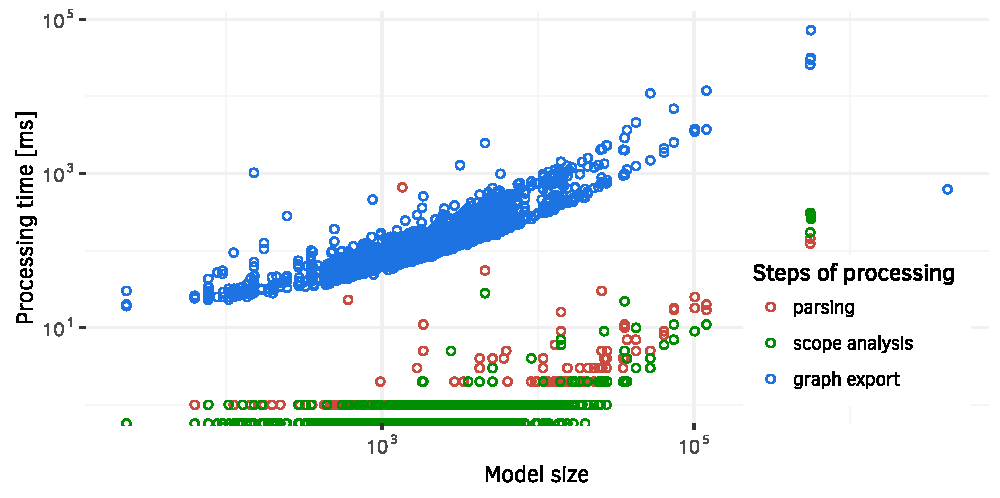
\includegraphics[width=\textwidth]{import-steps.pdf}
  \caption{The characteristics of the import steps.}
  \label{fig:import-steps}
\end{figure}

\Cref{fig:import-steps} shows the characteristics of these three steps. Since even the longest source codes can be written in one line, instead of the source lines of code I have chosen the number of nodes in the transformed subgraph (model size) as the horizontal axis. The vertical axis represents the time (in milliseconds) required to perform the given transformation step. Note that both axes are logarithmic.

In order to present an accurate and wide-range measurement, I have selected the repository of the Tresorit web client~\cite{tresorit-webclient}. The current version of this repository contains 780 JavaScript files, with 75\,907 lines of actual code in total. This results in 8\,437\,838 graph nodes.

Since the source code contains language elements not yet standardized, I translated the source code to conform ES5 before it is parsed by the Shift parser. This step is not calculated in the benchmark. The resulting files are then imported into the database one-by-one, sequentially, thus the parallel optimizations are not present in this measurement.

Based on~\Cref{fig:import-steps} the time requirement of the parsing and scope analysis steps are negligible compared to the third step. Iterating and storing the elements of the ASG in the graph database shows polynomial correlation with the size of the graph. It is also visible that most of the files are parsed under one second, which indicates that it can be employed in continuous and everyday development.

These results are based on two separate, sequential, full import of the source code repository, containing 780 files.

%\subsection{Connecting the Subgraphs}
% TODO write or hide

\subsection{Dead Code Search}
Searching for dead code snippets consists of two phases: first, the call graph has to be prepared, then the graph is queried for unreachable code. Since the transformation rules and queries are far from complete and are not covering every code model scenario, this measurement can only report the characteristics of the current implementation.

\begin{figure}[!htb]
  \centering
  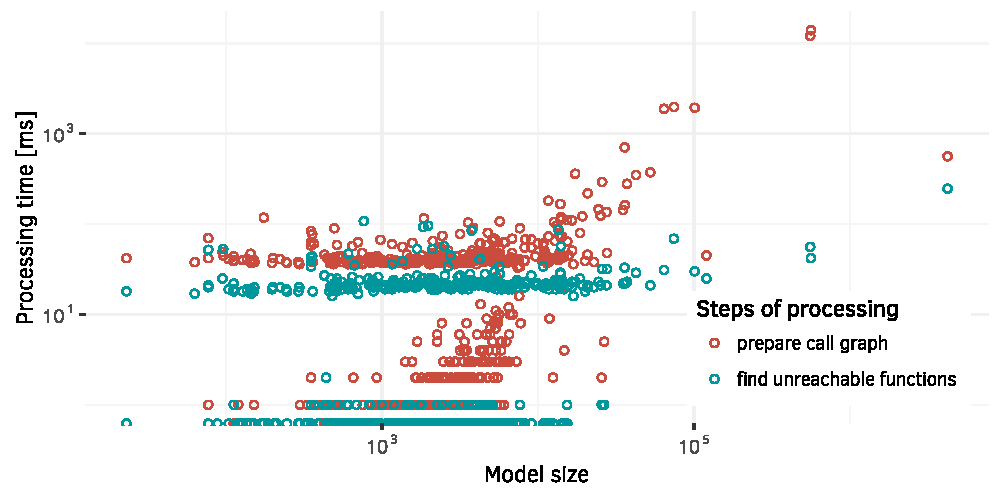
\includegraphics[width=\textwidth]{deadcode-search.pdf}
  \caption{The characteristics of dead code search.}
  \label{fig:deadcode-search}
\end{figure}

\Cref{fig:deadcode-search} shows at least two horizontal clusters for both steps. On the bottom, there are files that probably contain none or only a few nodes processed by the queries. Based on the figure and manual testing, the characteristics of the upper cluster is to be expected when the transformation rules provide full coverage, resulting in constant runtime for most cases.

The results are based on one-time, file-by-file import and dead code search of the source code repository, containing 780 files.

\subsection{ASG to CFG Transformation}
In order to measure the characteristics of the CFG transformation, I have imported the source files of the Tresorit web client one-by-one and executed the CFG transformation queries at a time.

\begin{figure}[!htb]
  \centering
  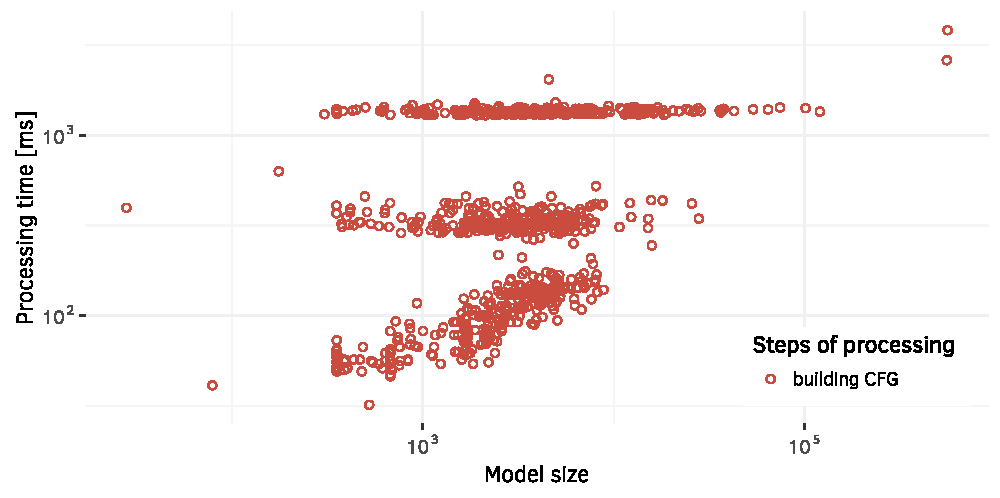
\includegraphics[width=\textwidth]{build-cfg.pdf}
  \caption{The characteristics of building the CFG.}
  \label{fig:build-cfg}
\end{figure}

\Cref{fig:build-cfg} shows that the measurements are clustered into three parts. There are at least two explanations for this:

\begin{itemize}[topsep=0pt]
  \item The number of CFG transformations implemented in the prototype framework is low. Since there are measurements in every cluster for a great amount of model sizes, it is possible that the composition of the files are different in each cluster.

  This would mean that the top cluster --- implementing business logic --- contains more nodes to transform, while the files in the bottom cluster --- mostly describing interfaces and proxies --- contain less.

  \item The transformation is executed in a parallel manner. If two transformations cause a deadlock in the database, they are canceled and tried again later. It is also possible that subgraphs containing more transformable nodes by the framework are processed slower. The slower the transformations are, the more deadlocks may happen, resulting in slower overall performance.
\end{itemize}

It is also unexpected to have the top two clusters show no correlation with the size of the resulting graph size. This phenomenon can be explained with the reasons above or with the way Neo4j executes declarative transformations.

The results are based on one-time, file-by-file import and transformation of the source code repository, containing 780 files. Since the CFG transformation in the framework is far from finished, deeper examination of the results is subject to future work.

\subsection{Incremental Processing}
Since the framework processes the changes file-by-file, it is possible to execute the analysis in an incremental fashion with file-level granularity. After every file has been processed and a new changeset is present, it is only required to update and process the modified file and the affected graph parts.

\begin{figure}[!htb]
  \centering
  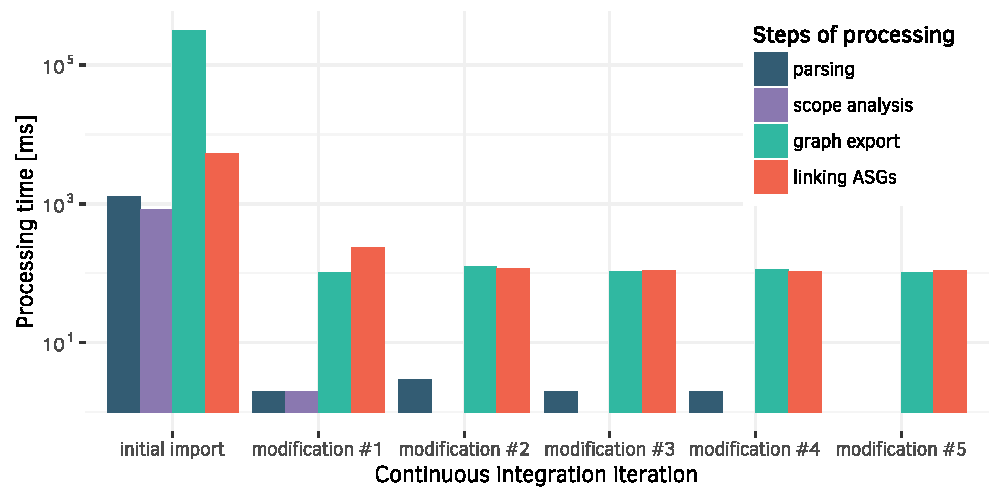
\includegraphics[width=\textwidth]{CI-iteration-benchmark.pdf}
  \caption{Runtime measurements of the execution of the analysis for sequential modifications.}
  \label{fig:CI-iteration-benchmark}
\end{figure}

\Cref{fig:CI-iteration-benchmark} details the execution times for each step during the initial and the subsequent change propagations. These all consist of the same steps: 1)~the source code is parsed, then 2)~scope analysis is applied, and 3)~the resulting ASG is stored in the graph database, finally 4)~the inserted subgraph is linked to the already stored nodes, imitating the JavaScipt module import-export resolution.

The initial import was executed first. After all 780 files have been processed one-by-one, the import-export linking was executed once. Subsequent modifications was simulated by removing and reprocessing a file with one of the most \code{import} statements (thus resulting in more work for the linking transformation). After each \emph{modification} the linking transformation was applied.

It is visible that the incremental approach for the complete process is faster by three orders of magnitude. The linking step itself is faster by one order of magnitude for linking only one file to the others. (Please note that along with the previous figures, \Cref{fig:CI-iteration-benchmark} is logarithmically scaled on the vertical axis.)


\section{IDE Integration}
\label{sect:ide-integration}
Besides executing measurements, I also created a plugin for Visual Studio Code (introduced in~\Cref{sect:visual-studio-code}) that sends the content of the open file to the framework, when the file is modified and saved. Then it requests the results of the dead code search, and conviniently displays it using the API provided by Visual Studio Code.

\begin{figure}[!htb]
  \centering
  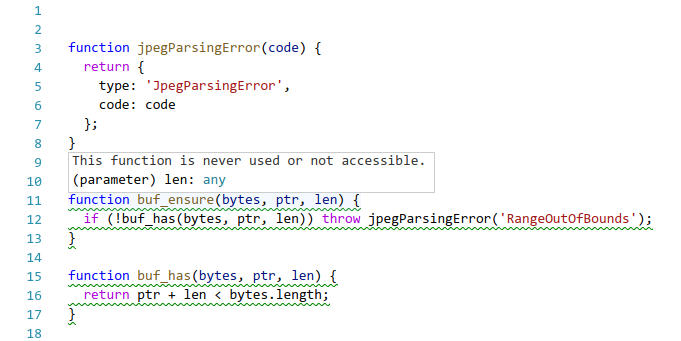
\includegraphics[width=\textwidth]{vsc-integration}
  \caption{Proof-of-concept plugin integration in an industrial case study.}
  \label{fig:vsc-integration}
\end{figure}

\Cref{fig:vsc-integration} shows the proof-of-concept plugin integration displaying dead code warnings for a file in an industrial case study. The previously introduced results in~\Cref{fig:dead-code-result} show that the approach was able to find circular references without incoming calls and report the clique, without user input. To validate the results, I have manually checked the presented warnings.


\section{Threats to Validity}
\label{sect:evaluation-threats}
Although I carefully designed and executed each measurement, there might have been factors beyond control that influence the results yielded. In this section, I try to list the possible mistakes and also discuss the steps taken to mitigate their effects.

\subsection{Benchmarking in the Cloud} As a multiple access system, the virtual servers in the cloud can be easily affected by neighboring virtual machines using the same resources. The virtual machine manager can also limit the usage of these resources, if the machines disturb other ones. One can neither control the resources assigned to the machines, nor influence their precise geolocation and connections.

My mitigation strategy is to run the benchmarks multiple times and treat their median as the representative value, or import a larger codebase with file sizes varying from a few to hundreds of lines.

\subsection{Methodological Mistakes} It is possible that I made mistakes while implementing the approach. It may not adhere to the specification correctly, perform the transformations correctly or measure correctly.

To check the validity of the results, I checked the results manually and with others tools.

\chapter{Future Vision}
\label{chap:future-vision}

My goal was to create the foundation of a versatile framework capable of doing even more than originally planned. Based on my approach there are several use-cases it makes possible:

\begin{itemize}[topsep=0pt]
  \item Existing linters do a good job at analyzing linting rules. However, extending them with new, complex rules is difficult. My approach allows tool developers to formalize rules more intuitively with graph patterns.

  \item With connecting the ASGs there are new possibilities in static analysis that were not possible or available before. This might be used for finding usages of source code elements, helping refactors and finding problematic structures reaching across files.

  \item Having several files processed in the same database also enables comparing them, potentially allowing executing sophisticated graph-based plagiarism searches.

  \item Transforming the ASG into CFG not only allows path searches, but combining it with other tools and techniques may result in automated test generation. This can result in higher code coverage and the more unresolved references discovered.

  \item Based on the CFG and the ASG, basic type inferencing algorithms may produce typing information in the untyped source code, allowing even more ways to write queries and constraints on the source code.
\end{itemize}

Since the transformation rules in the framework are far from finished, writing more, more precise, optimized, and general transformation rules and examining the benchmark results is subject to future work.

\chapter{Conclusions}
\label{chap:conclusions}

My main objective was and still is to provide a solution for reducing the time required for a global, codebase-level reevaluation of static analysis after a change occurs.

The elaborated framework can transform a rather large source code repository as a whole into a graph representation and maintain it subsequently. It is found that the approach is suitable for performing code convention compliance checks and for executing static analysis tests on the graph representation.

This approach also utilizes incremental processing with file-level granularity, speeding up the static analysis. Based on my measurements the framework is fast enough to help its users with fast changing code repositories.

Once the framework contains enough transformations and queries for handling the language, it can extend the everyday toolkit of developers.

\section{Summary of Contributions}
I presented an extensible proof of my novel concept to perform incremental static analysis on dynamic JavaScript source code repositories based on graph transformations. My proposal is based on software code modeling, graph transformation and graph pattern matching. The feasibility of the approach was evaluated using manual validation and benchmarking.

\subsection{Scientific Contributions}
I have achieved the following scientific contributions:

\begin{itemize}[topsep=0pt]
	\item Proposed an architecture for building an incremental static analyzer using freely available components.
	\item Proposed an approach to transform JavaScript source code repository into a connected graph model.
	\item Provided an algorithm to update the graph data model incrementally.
	\item Presented a working method for finding problematic code parts using graph pattern matching.
	\item Provided a transformation approach for creating CFG\footnote{Control Flow Graph} from ASG\footnote{Abstract Semantic Graph}.
\end{itemize}

\subsection{Practical Accomplishments}
I have also achieved the following practical accomplishments:

\begin{itemize}[topsep=0pt]
	\item Created an extensible incremental static analysis framework.
	\item Developed a tool for transforming JavaScript source code into graph data model.
	\item Designed a benchmark evaluating the approach.
\end{itemize}

\section{Novel Results}
Compared to my earlier work in static analysis~\cite{stein-daniel-tdk,stein-daniel-bsc,stein-daniel-ttc}, this report has the following novel contributions:

\begin{itemize}[topsep=0pt]
	\item This approach utilizes a property graph for storing the transformed model of the source code (as opposed to EMF\footnote{Eclipse Modeling Framework} and RDF\footnote{Resource Description Framework} models).

	\item My approach tackles the problem of carrying out static analysis for dynamic languages (e.g., JavaScript), instead of static languages (e.g., Java).

	\item Besides static analysis, I proposed an algorithm for transforming the ASG into a variant of the CFG.

	\item This approach was tested on an industrial case study, provided by Tresorit Kft.

	\item I have implemented a proof-of concept IDE integration with Visual Studio Code that is able to detect dead code with quick response times and display corresponding warnings to the source code developers.
\end{itemize}


\backmatter{}
\pagenumbering{roman}
\setcounter{page}{\thesavepage}

\chapter*{Acknowledgments}
\addcontentsline{toc}{chapter}{Acknowledgments}
\label{chap:acknowledgments}
\thispagestyle{plain}

First, I would like to thank Dr. István Ráth and Zoltán Ujhelyi for providing the scientific foundations for my research and insight into software model verification.

I would like to thank my supervisors Ádám Lippai, Dávid Honfi, and Gábor Szárnyas for their friendly advice and enthusiasm. Also, I wish to express my gratitude to all other colleagues at Tresorit and the Fault Tolerant Systems Research Group who provided numerous valuable observations and suggestions.

Last but not least, I am deeply grateful to my family and friends for their continuous support.


%\section*{Awards}
%I am also thankful for the two awards supporting my work.
\vfill

\paragraph{Microsoft Azure for Research Award}
This report was supported by Microsoft Azure making it possible to use cloud resources with ease.

\paragraph{New National Excellence Program}
This report was supported by the ÚNKP-16-2-I. New National Excellence Program of the Ministry of Human Capacities.

\begin{center}

\includegraphics[width=0.3\textwidth]{include/figures/min_en.jpg}
\end{center}


\listoffigures*\addcontentsline{toc}{chapter}{List of Figures}
\listoftables*\addcontentsline{toc}{chapter}{List of Tables}

\printbibliography{}

\appendix
\chapter*{Appendix}\addcontentsline{toc}{chapter}{Appendix}


\label{page:last}

\end{document}
